%Title: Beamer Presentation Template
%Author: LISA
%Year: 2020

\documentclass[10pt,aspectratio=169]{beamer}
 
%
%Setting file
%

\usepackage[T1]{fontenc}
\usepackage[utf8]{inputenc}

\usepackage[english]{babel}

\usepackage{graphicx}
\graphicspath{{images/}}
\usepackage{float}
\usepackage{tikz}
\usepackage{caption}
\usepackage{subcaption}

\usetheme{default}
\usefonttheme{structurebold}


% ---------------------------------
% color definitions
\usepackage{color}
% \definecolor{LISA_BLUE}{rgb}{0.25,0.33,0.66}
\definecolor{LISA_BLUE}{cmyk}{0.99,0.88,0.29,0.18}

\setbeamercolor{normal text}{fg=LISA_BLUE}
\setbeamercolor{frametitle}{fg=LISA_BLUE}

\newcommand\insertlocation{}  % Empty by default.
\newcommand\location[1]{\renewcommand\insertlocation{#1}}

\newcommand\insertperiod{}  % Empty by default.
\newcommand\period[1]{\renewcommand\insertperiod{#1}}



\setbeamertemplate{itemize items}[circle]
\setbeamercolor{title}{fg=white}



%-----------------------------------------Title page settings-----------------------------------------%
\title{Proton-induced fusion-evaporation reactions for actinide production at IGISOL}
\subtitle{}
\author{\small A. Raggio$^{1}$, I. Moore$^{1}$, I. Pohjalainen$^{2}$, \\ E. Rey-Herme$^{3}$, J. Saren$^{1}$, M. Vandebrouck$^{3}$}
\institute{$^{1}$ Jyv\"{a}skyl\"{a} University \\
$^{2}$ GSI Helmholtzzentrum für Schwerionenforschung GmbH\\
$^{3}$ CEA, Universite Paris-Saclay}
\period{}
\date{May 26-28, 2021}
\location{Event}


%-----------------------------------------Title page settings-----------------------------------------%


\begin{document}

{
  \usebackgroundtemplate{
\includegraphics[width=\paperwidth]{Title.pdf}}
	\begin{frame}[noframenumbering, plain]
		\titlepage
	\end{frame}
}
%----------------------------Content---------------------------------
\begin{frame}{Content}
	\begin{textblock*}{0.5\paperwidth}(0.03\paperwidth,0.18\paperheight)
		\begin{itemize}
			\item[]<1->{Physics Case\\
			\begin{itemize}
				\item Optical Spectroscopy
				\item A test bench for collective behavior
			\end{itemize}
			}
			\vspace{0.02\textheight}
			\item[]<2->{Actinide Quest at IGISOL\\
					\begin{itemize}
						\item Production
						\item Collinear Laser Spectroscopy
						\item Decay Spectroscopy
					\end{itemize}
					}
			\vspace{0.02\textheight}
			\item[]<3->{Proton-induced Fusion-evaporation\\ with actinide targets\\
					\begin{itemize}
						\item A decay spectroscopy experiment\\ with $^{232}$Th target
						\item Production Yield
						\item Combination with Penning Trap measurements
					\end{itemize}
					}
		\end{itemize}
	\end{textblock*}
	\begin{textblock*}{0.5\paperwidth}(0.47\paperwidth,0.2\paperheight)
		% \vspace{0.1\textheight}
		\only<1>{\includegraphics[width=\textwidth]{Full_Chart.pdf}}%
		\only<2>{\vspace{0.2\textheight}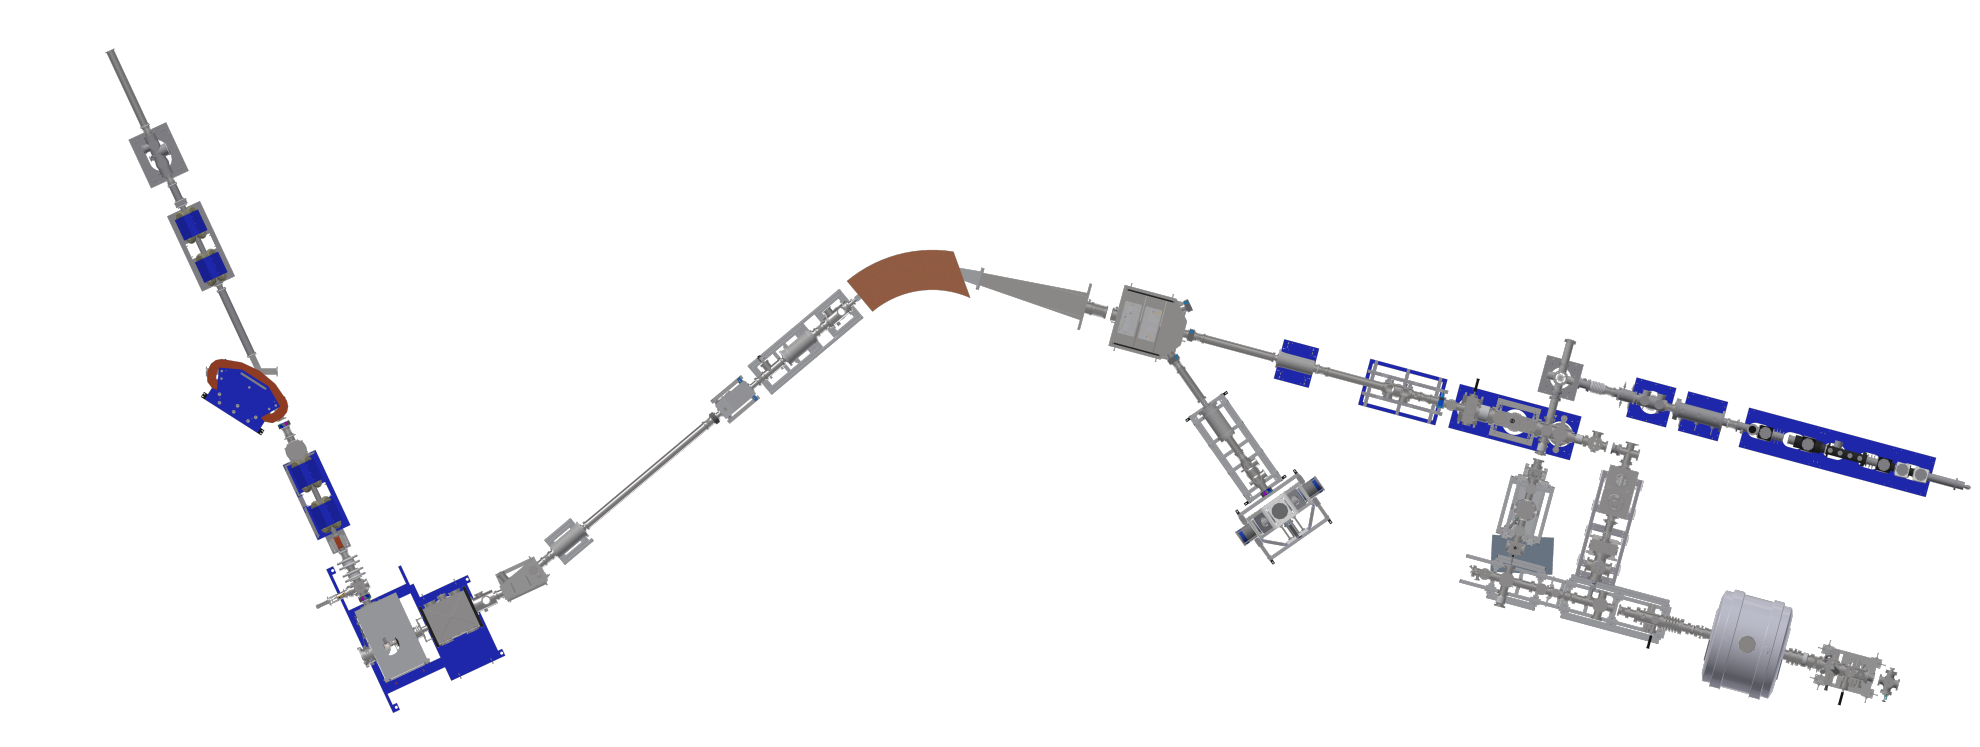
\includegraphics[width=\textwidth]{IGI-1A-IGISOL_3_no_logo.png}}%
		\only<3>{\vspace{0.2\textheight}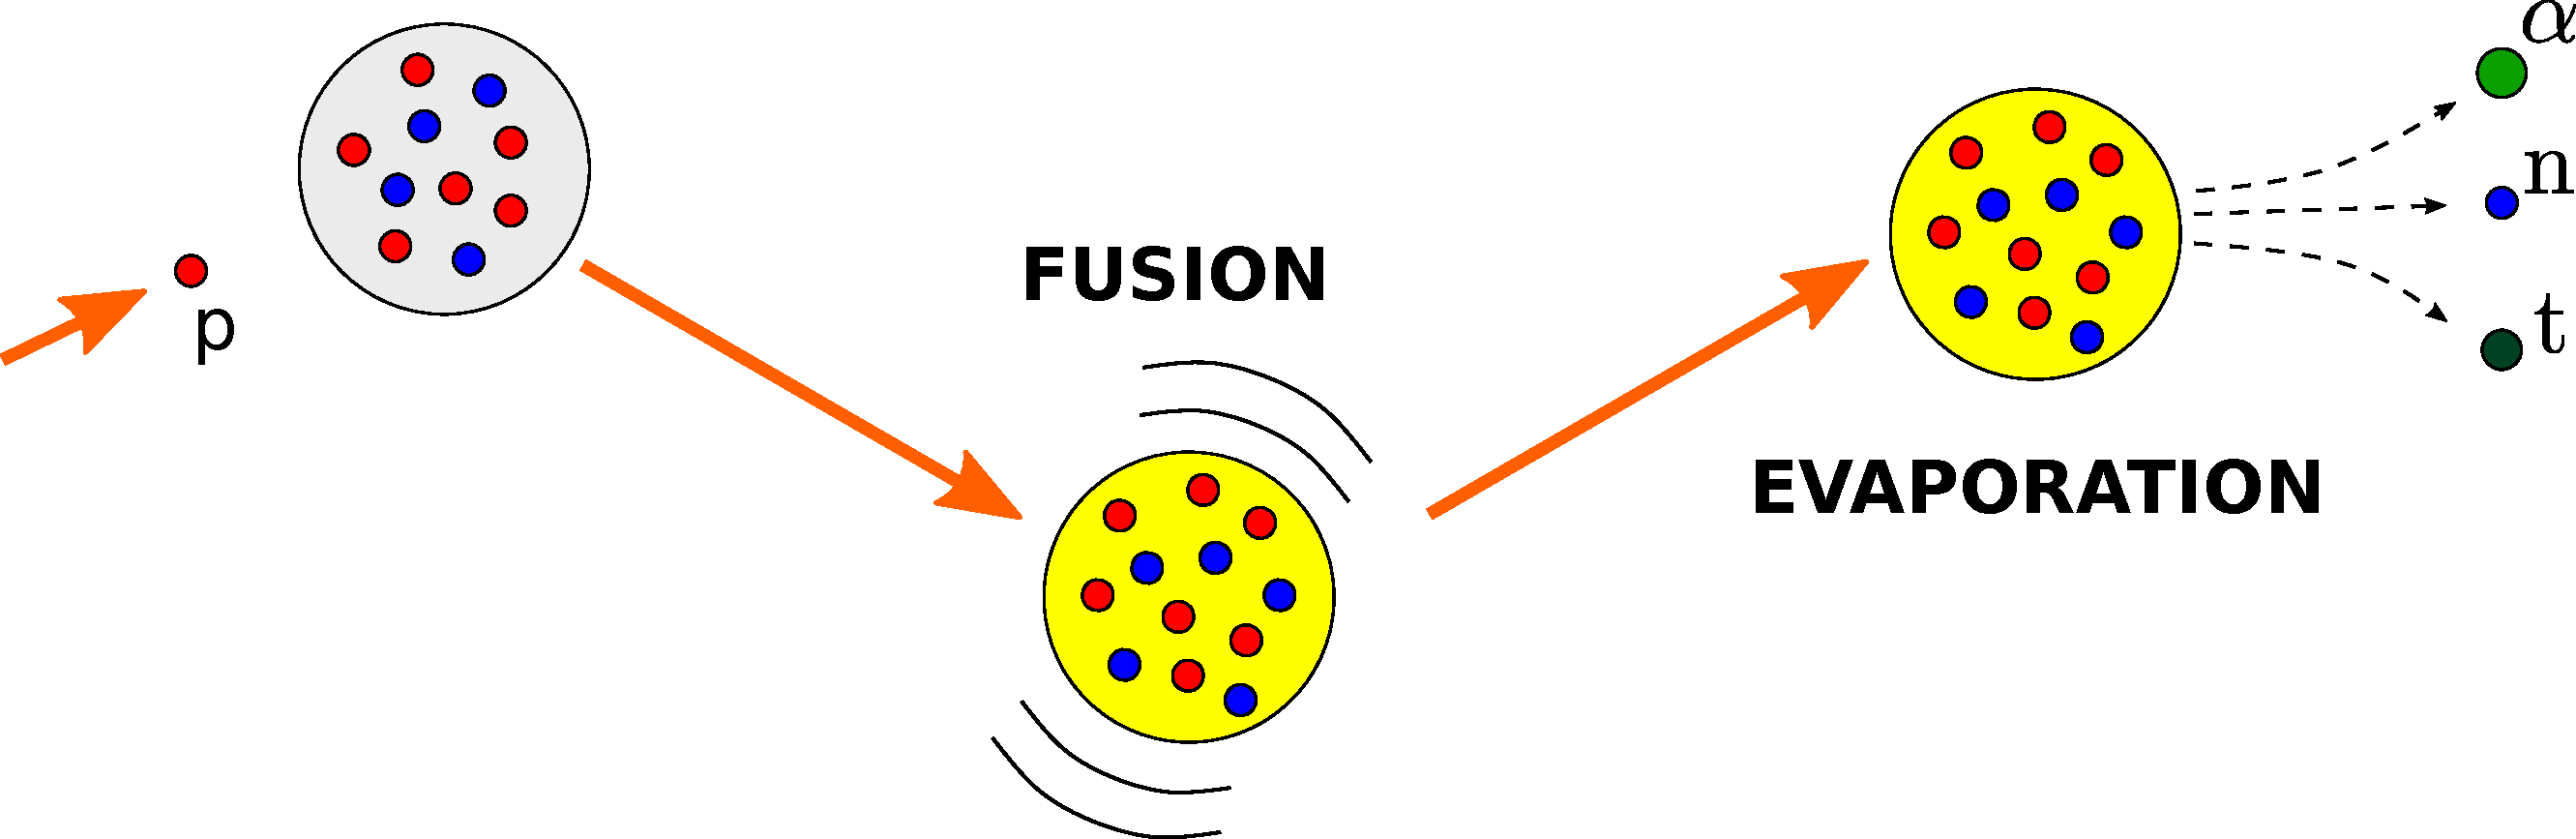
\includegraphics[width=\textwidth]{Reaction.pdf}}%
	\end{textblock*}
\end{frame}

%----------------------------Motivation---------------------------------
\begin{SectionTitle}
\begin{frame}
	\centering
	\begin{textblock*}{0.5\paperwidth}(0.25\paperwidth,0.15\paperheight)
		\centering
		\textbf{\LARGE PHYSICS CASE}	
	\end{textblock*}
	\begin{textblock*}{0.5\paperwidth}(0.25\paperwidth,0.3\paperheight)
        \includegraphics[width=.8\textwidth]{Full_Chart.pdf}
	\end{textblock*}

\end{frame}
\end{SectionTitle}

\begin{frame}{Optical Spectroscopy on Actinides}
	\begin{textblock*}{0.5\paperwidth}(0.015\paperwidth,0.18\paperheight)
		\begin{textblock*}{0.1\paperwidth}(0.05\paperwidth,0.7\paperheight)
			\footnote{Updated from P. Campbell et al., PPNP 86 (2016) 127–180}
		\end{textblock*}
		\only<1>{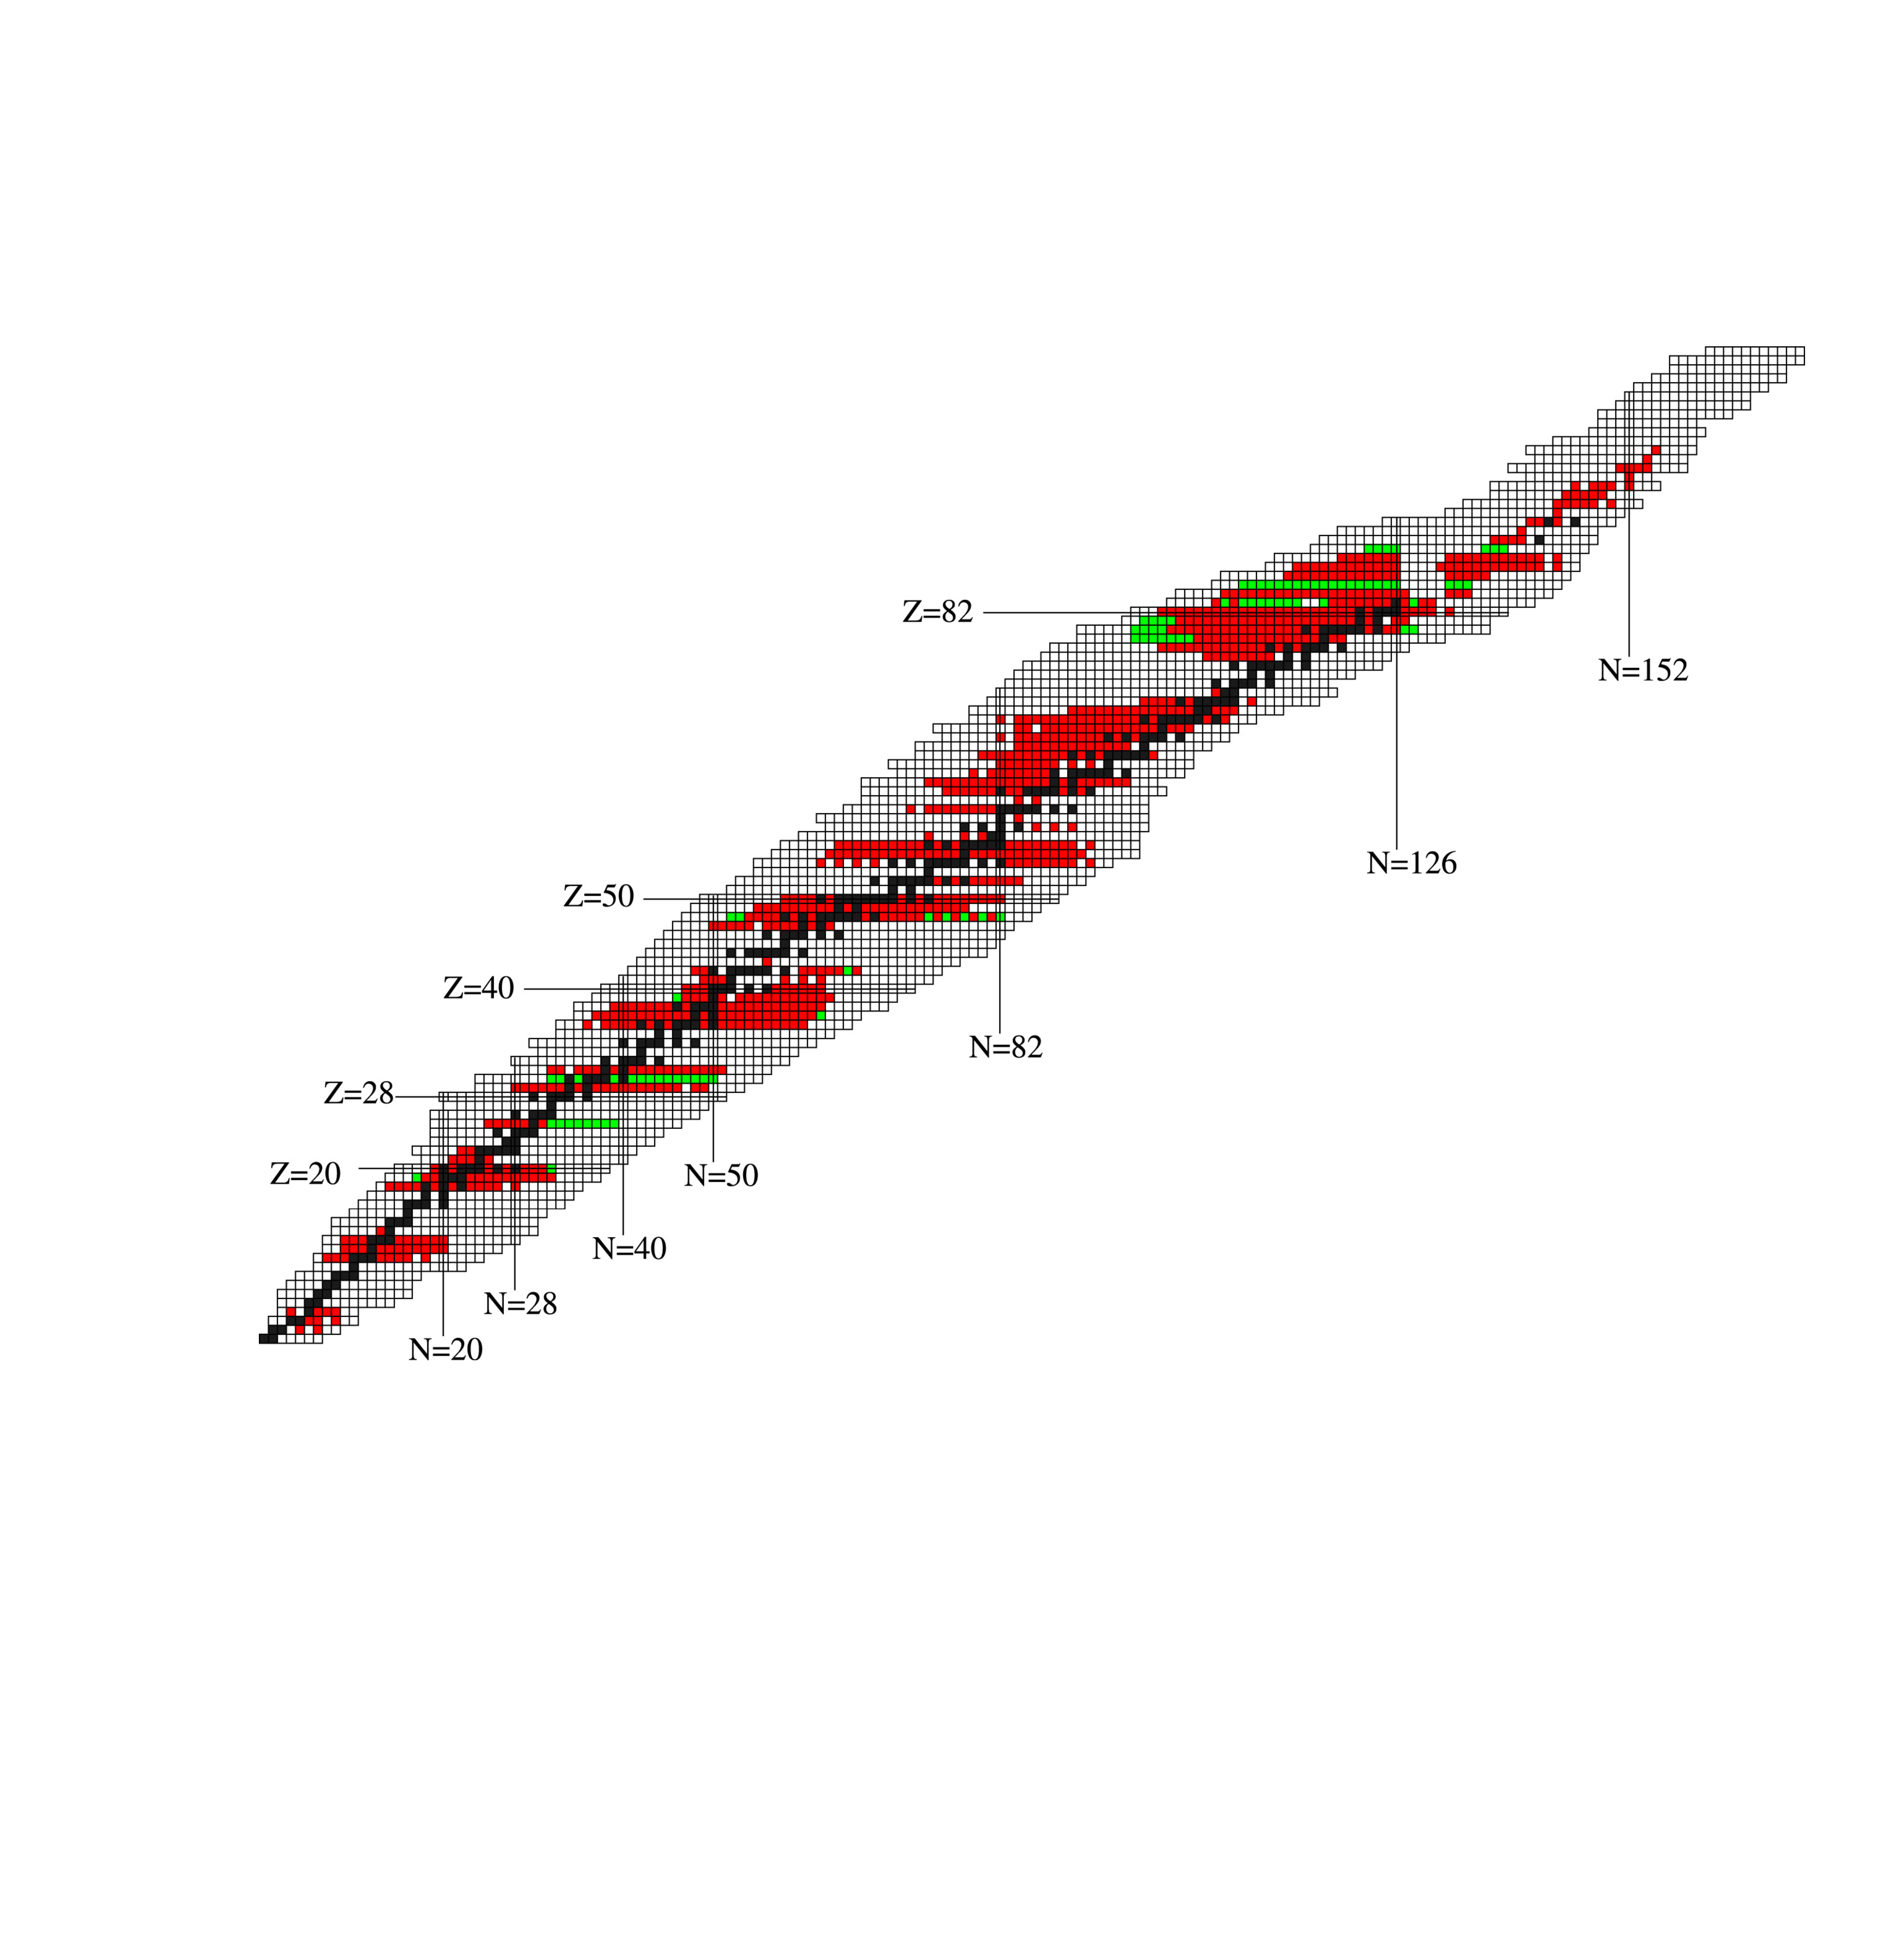
\includegraphics[width=0.8\textwidth]{AChart_0.pdf}}%
        \only<2>{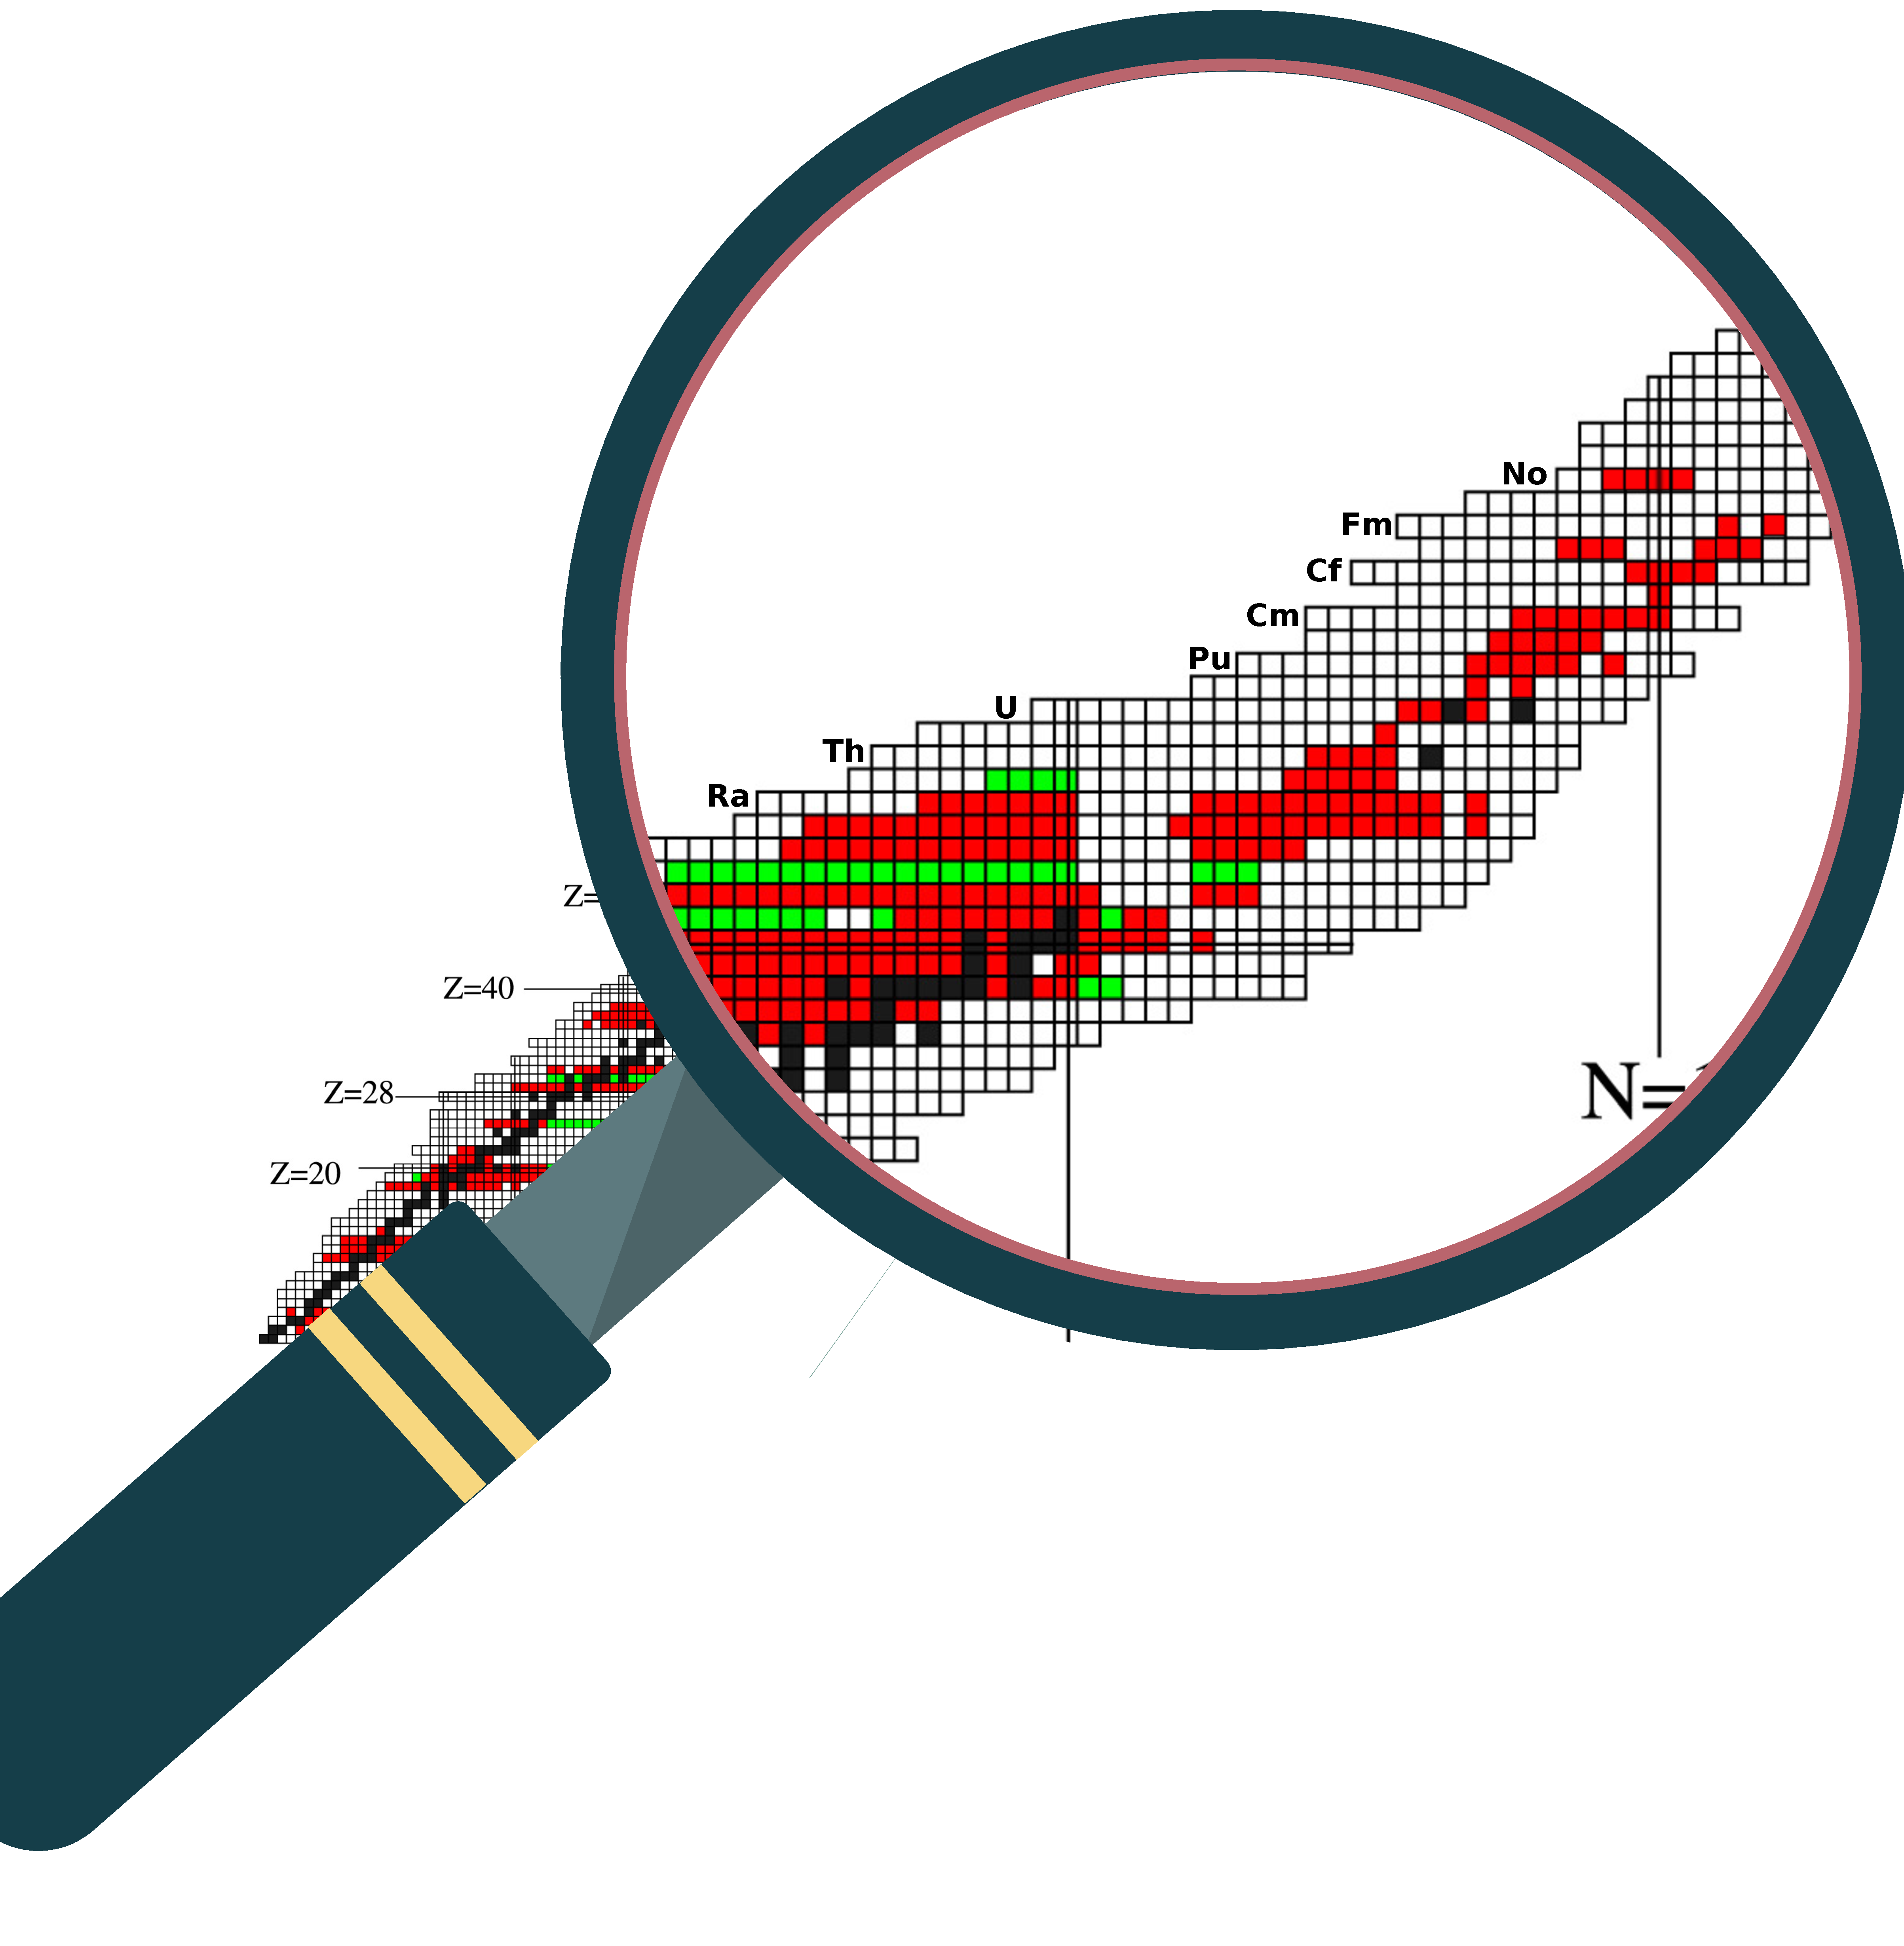
\includegraphics[width=0.8\textwidth]{AChart_1.pdf}}%
	\end{textblock*}
	\only<2->{
	\begin{textblock*}{0.6\paperwidth}(0.4\paperwidth,0.18\paperheight)
		\centering
		A usefull tool to exctract fundamental nuclear properties
	\end{textblock*}
	\begin{textblock*}{0.4\paperwidth}(0.65\paperwidth,0.25\paperheight)
		\textbf{General lack of optical data}
		\begin{itemize}
			\item Lack of Stable isotopes
			\item Challenging Production
		\end{itemize}
	\end{textblock*}		
	\begin{textblock*}{0.3\paperwidth}(0.46\paperwidth,0.27\paperheight)
		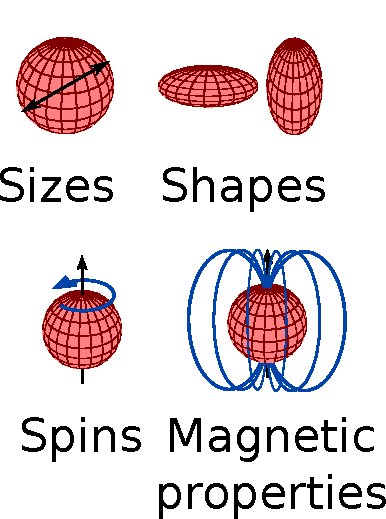
\includegraphics[width=0.5\textwidth]{shapes.pdf}
	\end{textblock*}
	\begin{textblock*}{0.4\paperwidth}(0.6\paperwidth,0.45\paperheight)
		\centering
		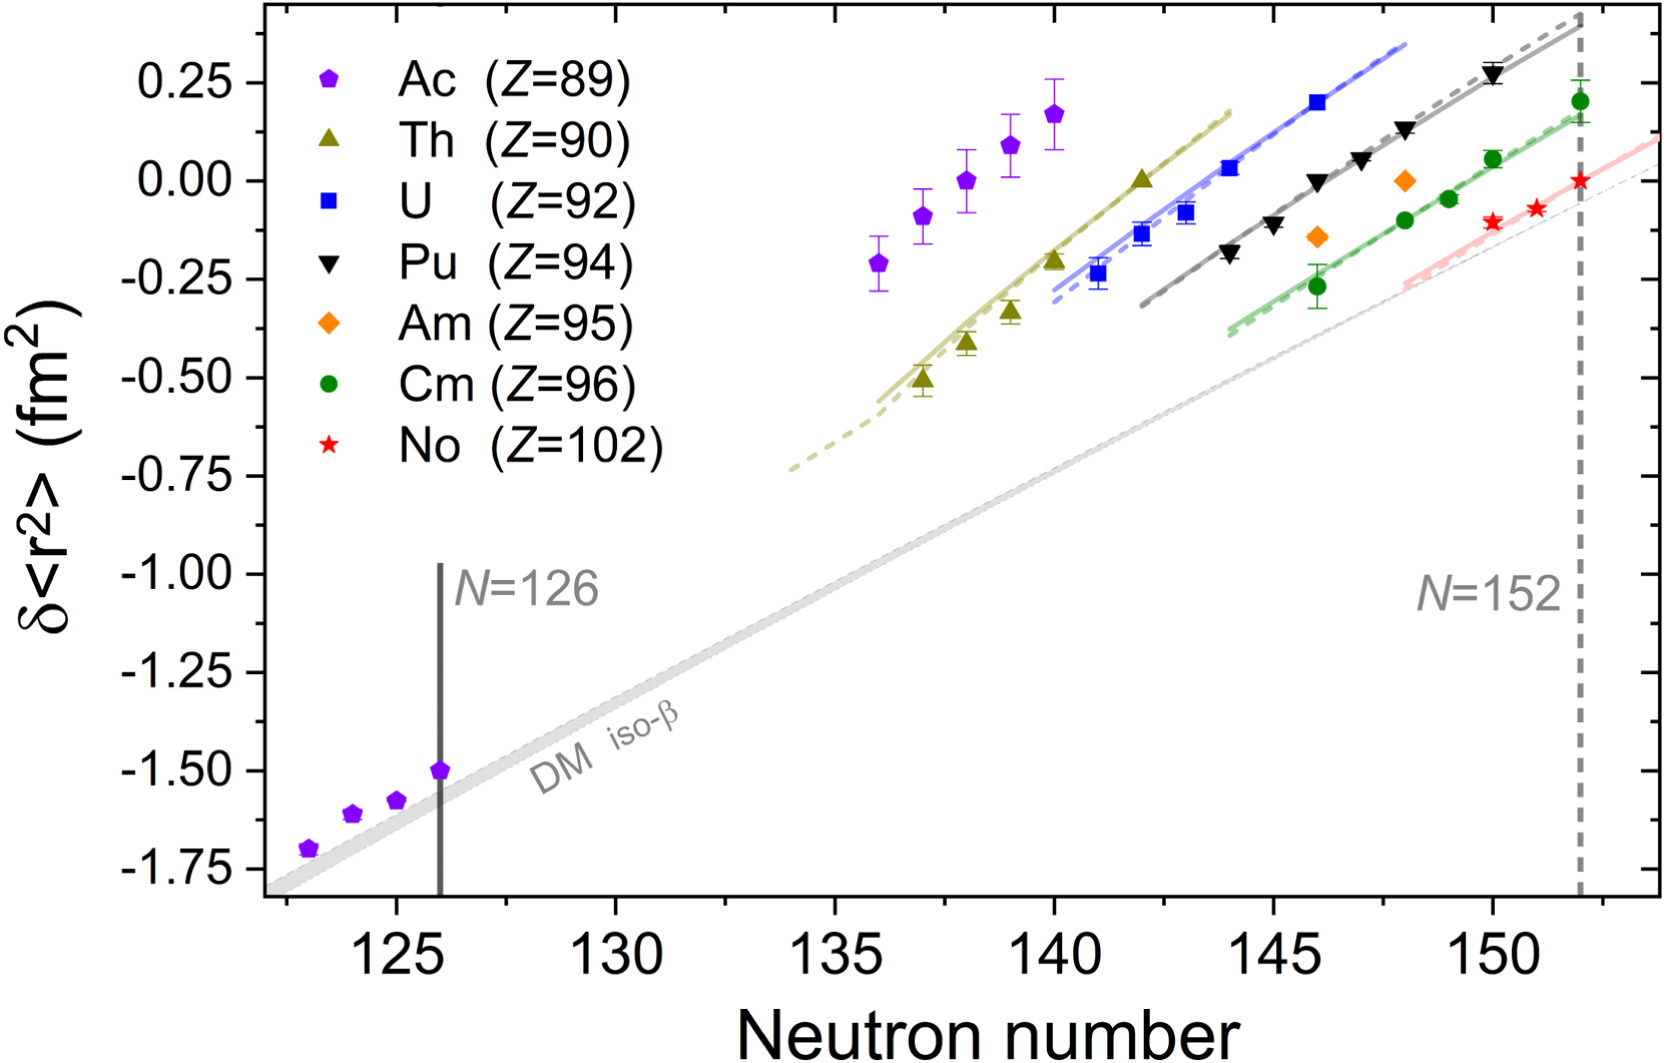
\includegraphics[width=0.8\textwidth]{MSCR.jpg}
		\footnote{M. Block et al., PPNP, 116 (2021), 103834}
	\end{textblock*}
	\begin{textblock*}{0.4\paperwidth}(0.3\paperwidth,0.75\paperheight)
		\textbf{Model-indipendent measurement} 
	\end{textblock*}}
\end{frame}

\begin{frame}{Octupole Deformation and Charge Radii}
	\begin{textblock*}{0.9\paperwidth}(0.05\paperwidth,0.18\paperheight)
		\centering
		$\langle r^2 \rangle = \langle r^2 \rangle_{sph} \left( 1+\dfrac{5}{4 \pi}\left( \langle \beta^2_2\rangle+\langle \beta^2_3\rangle+...\right)\right)$
	\end{textblock*}
	\begin{textblock*}{0.4\paperwidth}(0.01\paperwidth,0.26\paperheight)
		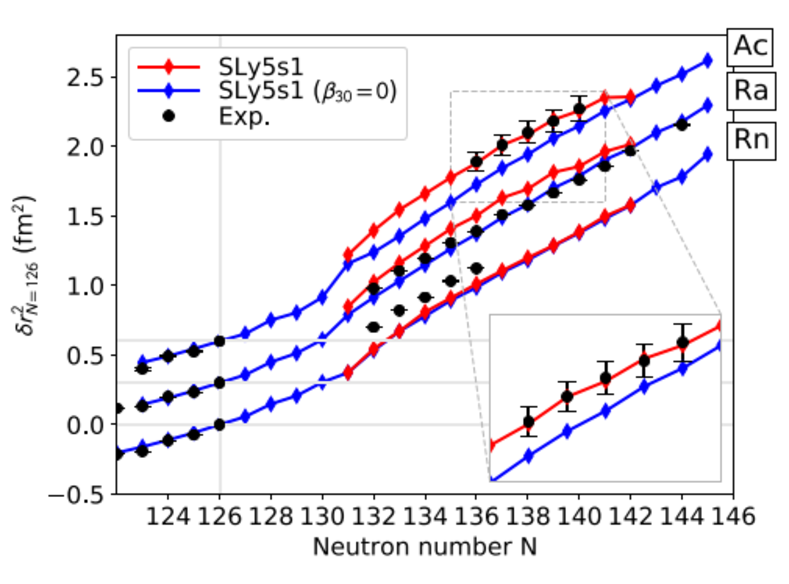
\includegraphics[width=\textwidth]{OctupoleBeta.pdf}
	\end{textblock*}
	\begin{textblock*}{0.1\paperwidth}(0.4\paperwidth,0.75\paperheight)
		\footnote{Y. Cao et al., Phys. Rev. C 102 (2020) 024311}
	\end{textblock*}
	\begin{textblock*}{0.15\paperwidth}(0.4\paperwidth,0.26\paperheight)
		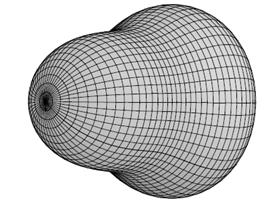
\includegraphics[width=\textwidth,angle=45]{OctupolePear.jpg}
	\end{textblock*}
	\begin{textblock*}{0.4\paperwidth}(0.6\paperwidth,0.28\paperheight)
		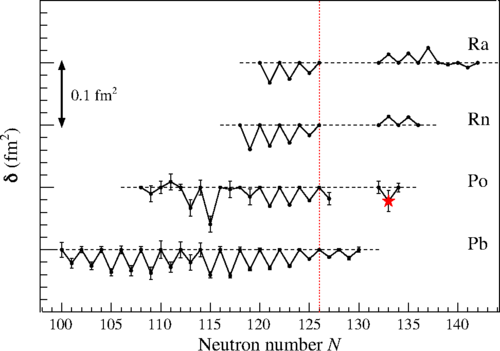
\includegraphics[width=0.7\textwidth]{OddEven.png}
	\end{textblock*}
	\begin{textblock*}{0.1\paperwidth}(0.9\paperwidth,0.62\paperheight)
		\footnote{D. Fink et al., PRX 5 (2015) 011018}
	\end{textblock*}
	\begin{textblock*}{0.6\paperwidth}(0.4\paperwidth,0.62\paperheight)
		\small	
		\begin{itemize}
				\item Comparison with EDF predictions. 
				\item Need to extend to heavier actinide experimental data
				\item Correlation between odd-even staggering reversal and octupole deformation?
			\end{itemize}
	\end{textblock*}
\end{frame}


%----------------------------IGISOL---------------------------------
\begin{SectionTitle}
	\begin{frame}
		\centering
		\begin{textblock*}{0.5\paperwidth}(0.25\paperwidth,0.15\paperheight)
			\centering
			\textbf{\LARGE ACTINIDE QUEST AT IGISOL}	
		\end{textblock*}
		\begin{textblock*}{0.5\paperwidth}(0.25\paperwidth,0.4\paperheight)
			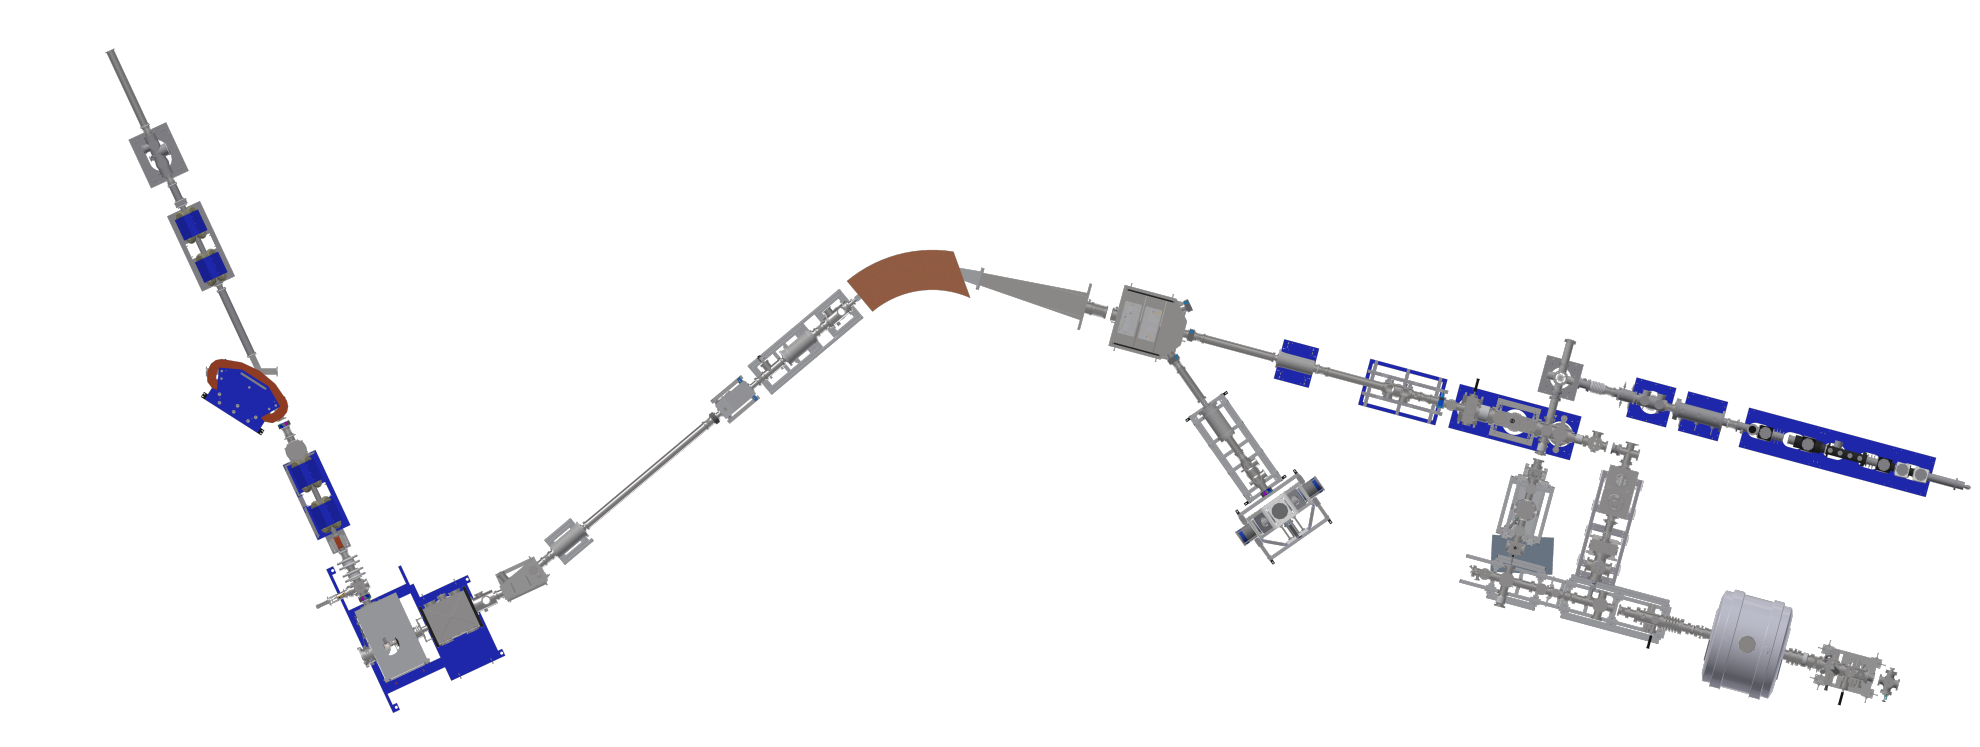
\includegraphics[width=.9\textwidth]{IGI-1A-IGISOL_3_no_logo.png}
		\end{textblock*}
	\end{frame}
\end{SectionTitle}
	
\begin{frame}{Offline Production}
	\begin{textblock*}{0.8\paperwidth}(0.01\paperwidth,0.1\paperheight)
		\only<1->{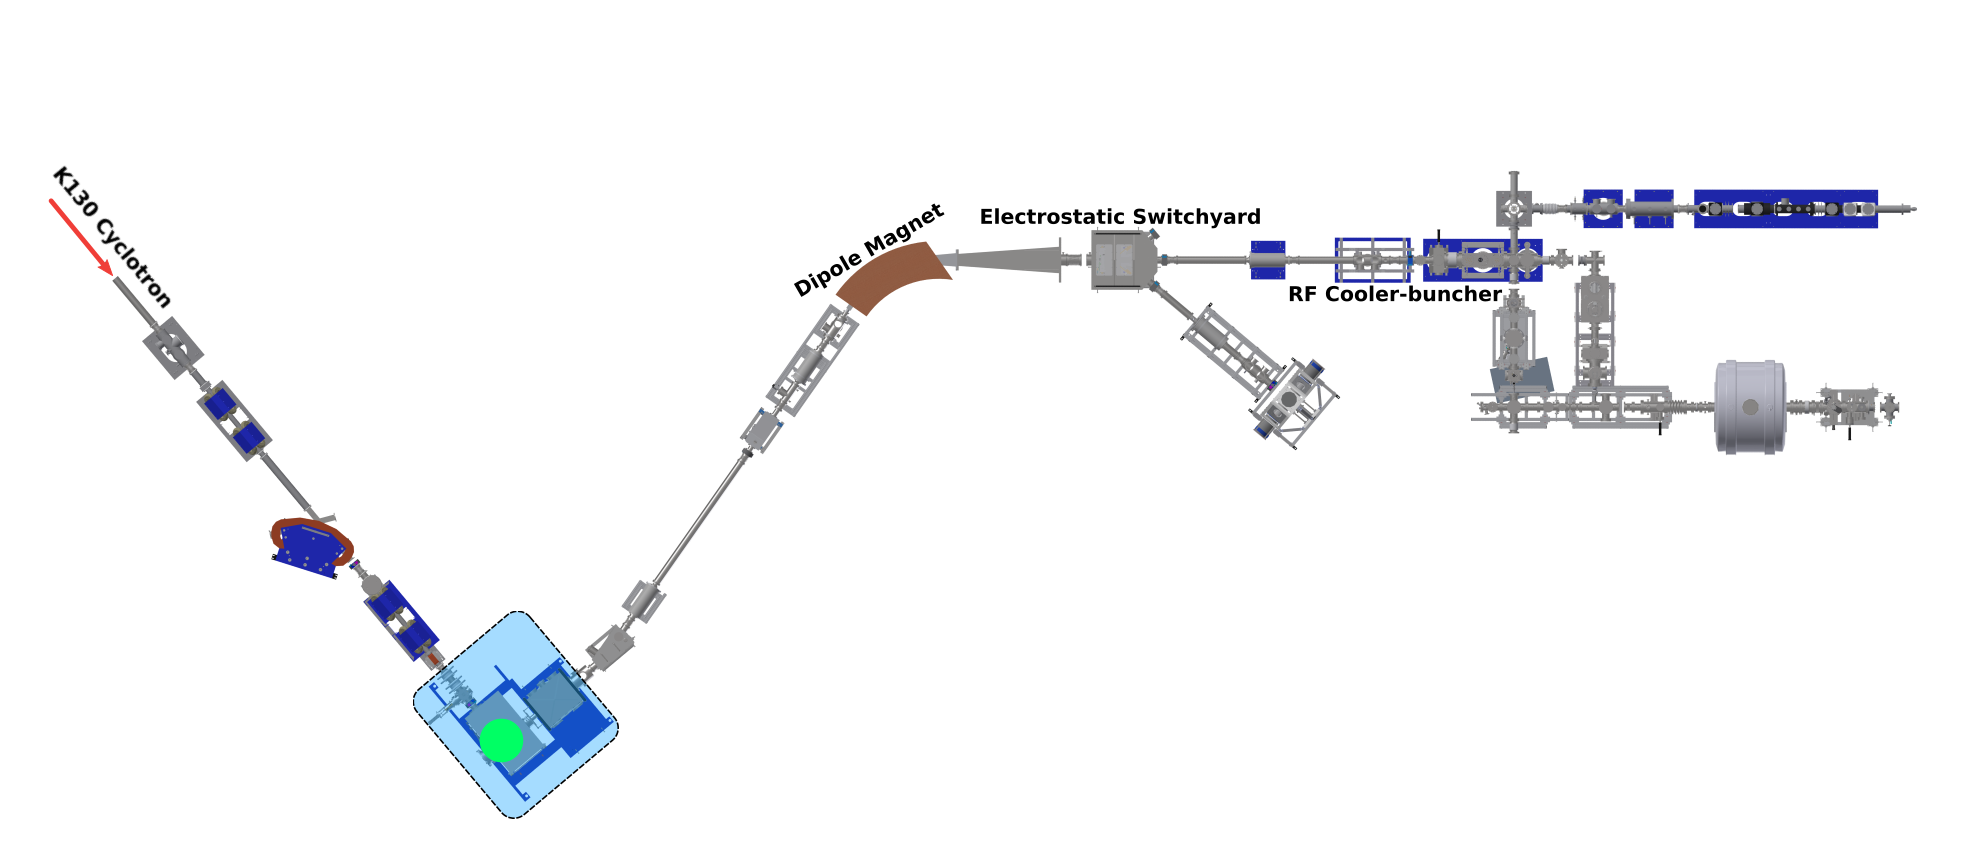
\includegraphics[width=\textwidth]{Igisol_scheme_TG.png}}%
		% \only<1>{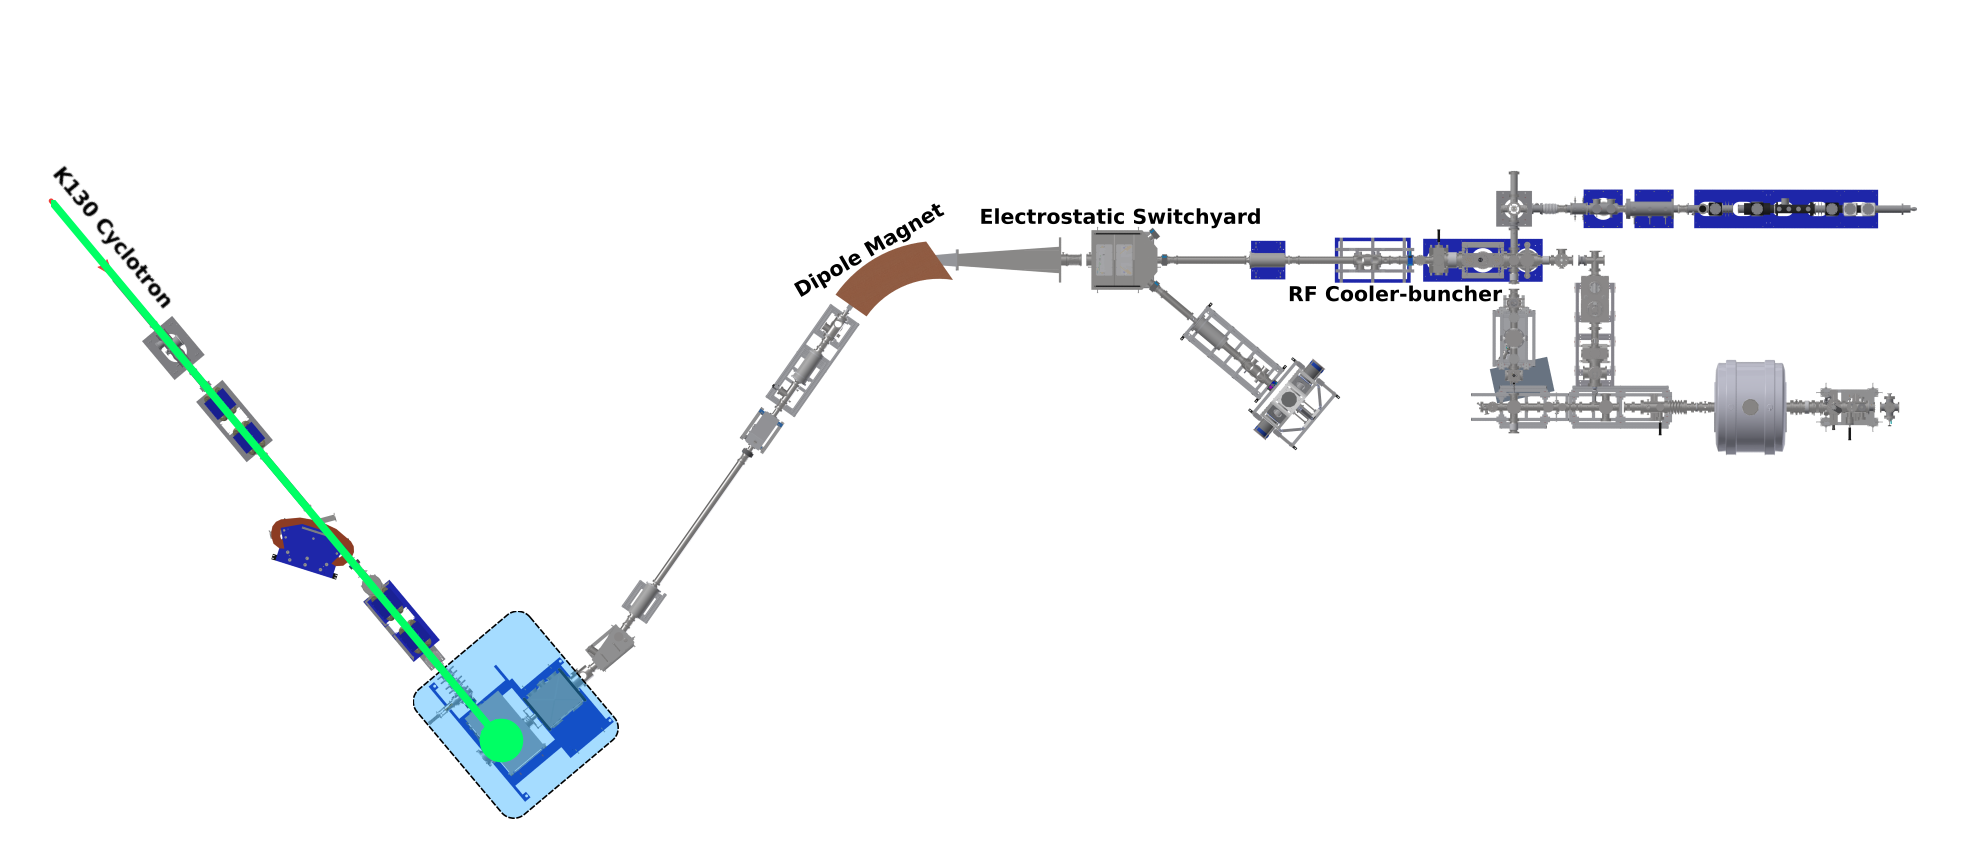
\includegraphics[width=\textwidth]{Igisol_scheme_TG_online.png}}%
		% \only<4>{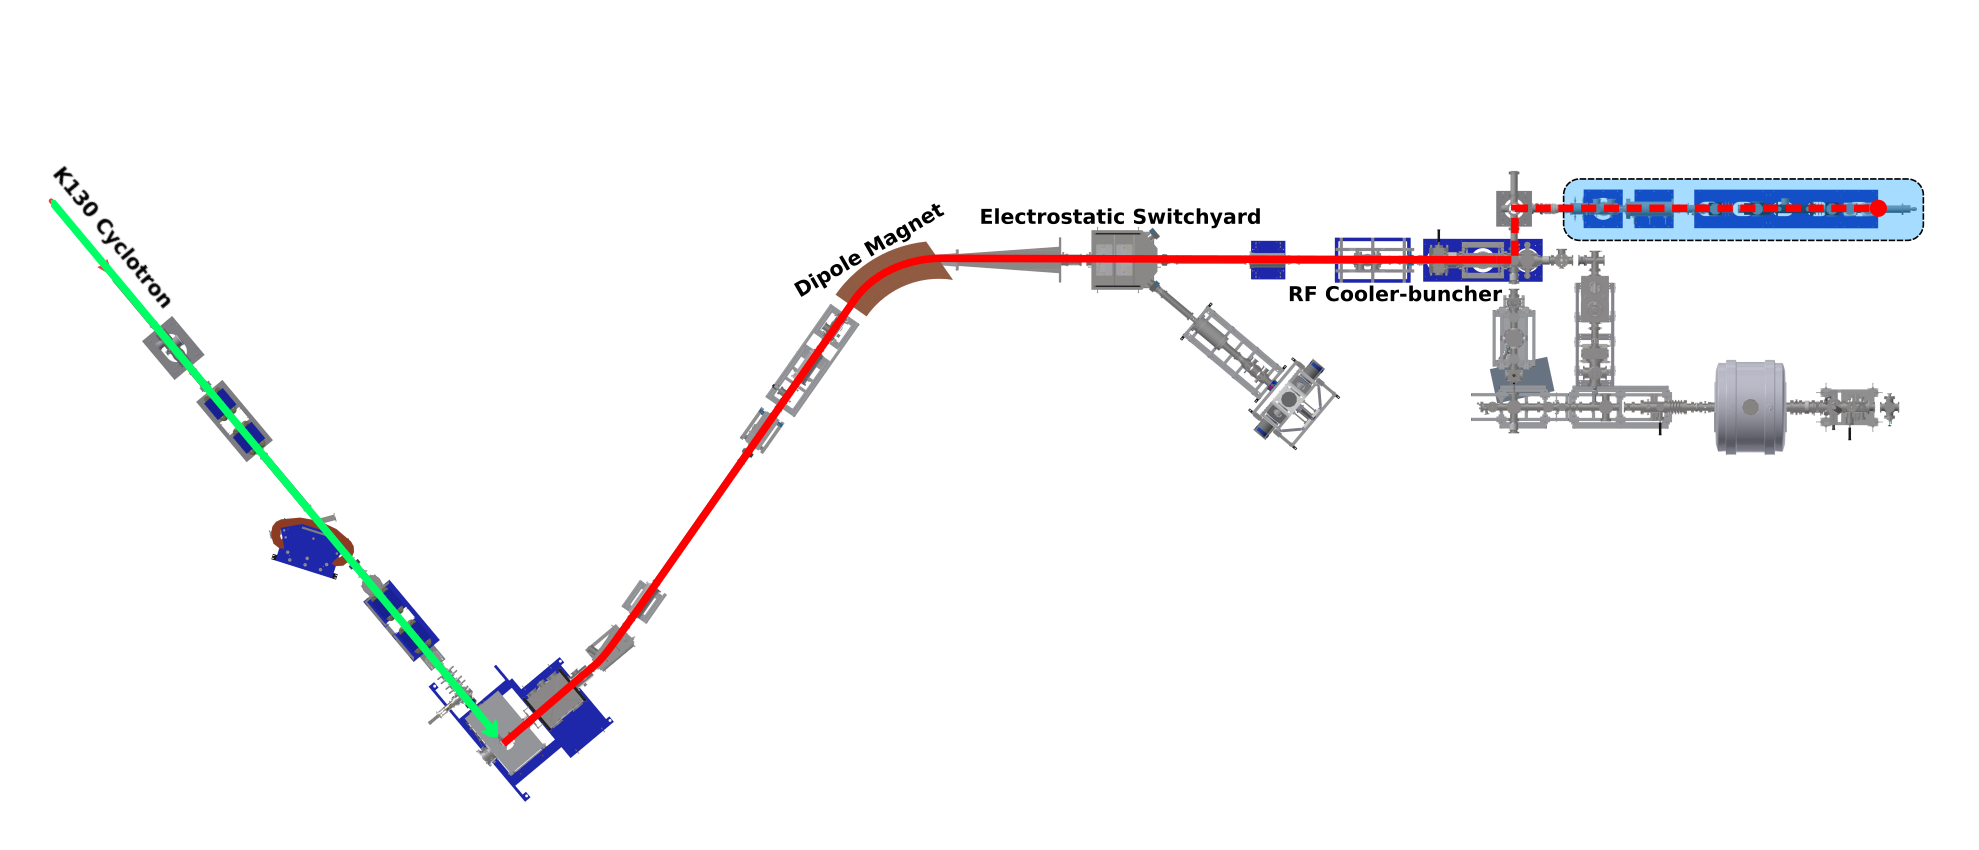
\includegraphics[width=\textwidth]{Igisol_scheme_CLS.png}}%
		% \only<5>{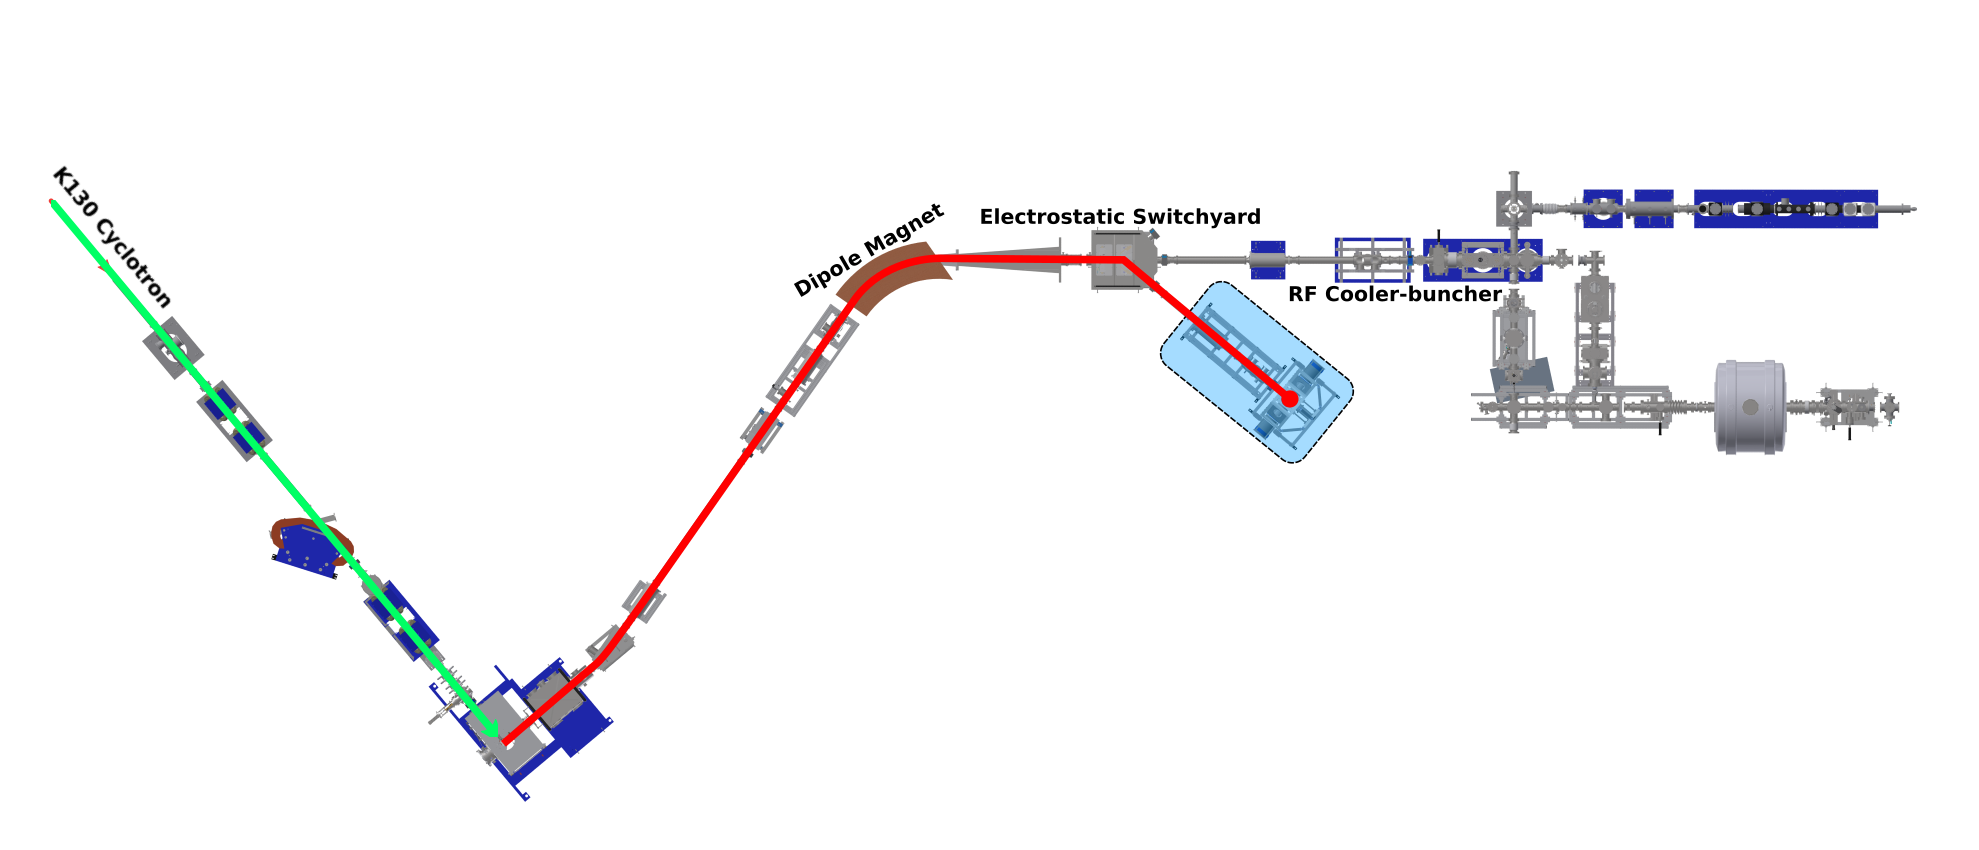
\includegraphics[width=\textwidth]{Igisol_scheme_Spec.png}}%
		% \only<6>{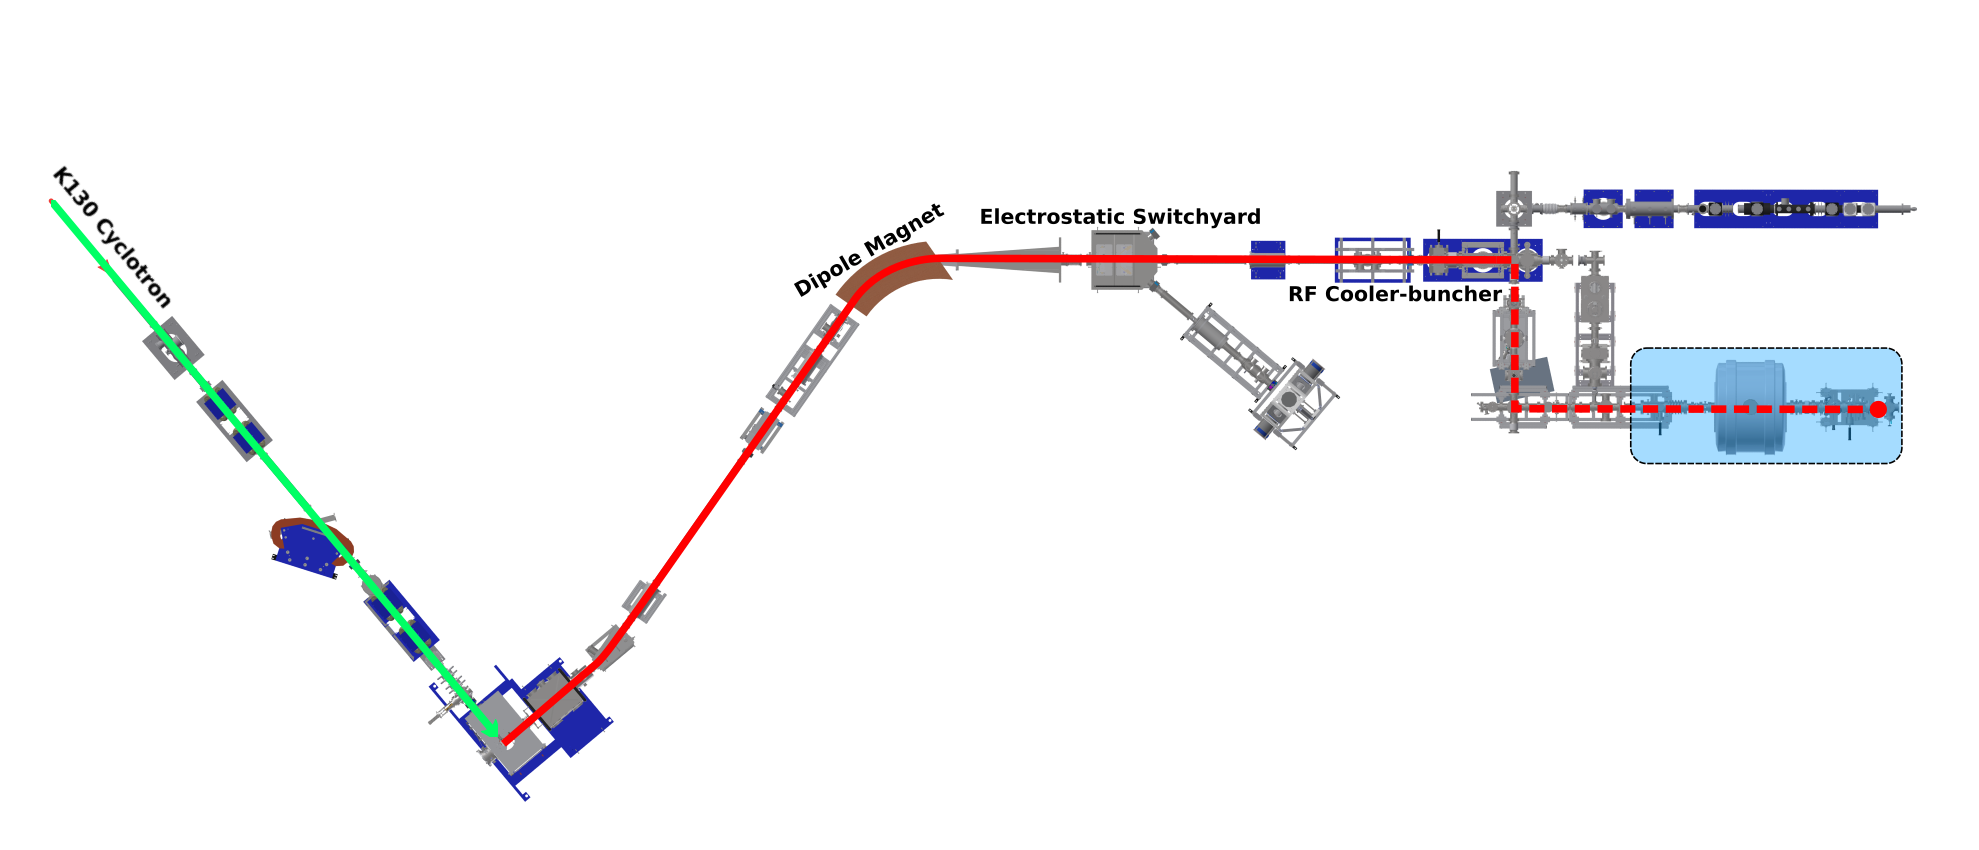
\includegraphics[width=\textwidth]{Igisol_scheme_Penn.png}}%
	\end{textblock*}
	\only<1>{
		\begin{textblock*}{0.185\paperwidth}(0.13\paperwidth,0.17\paperheight)
			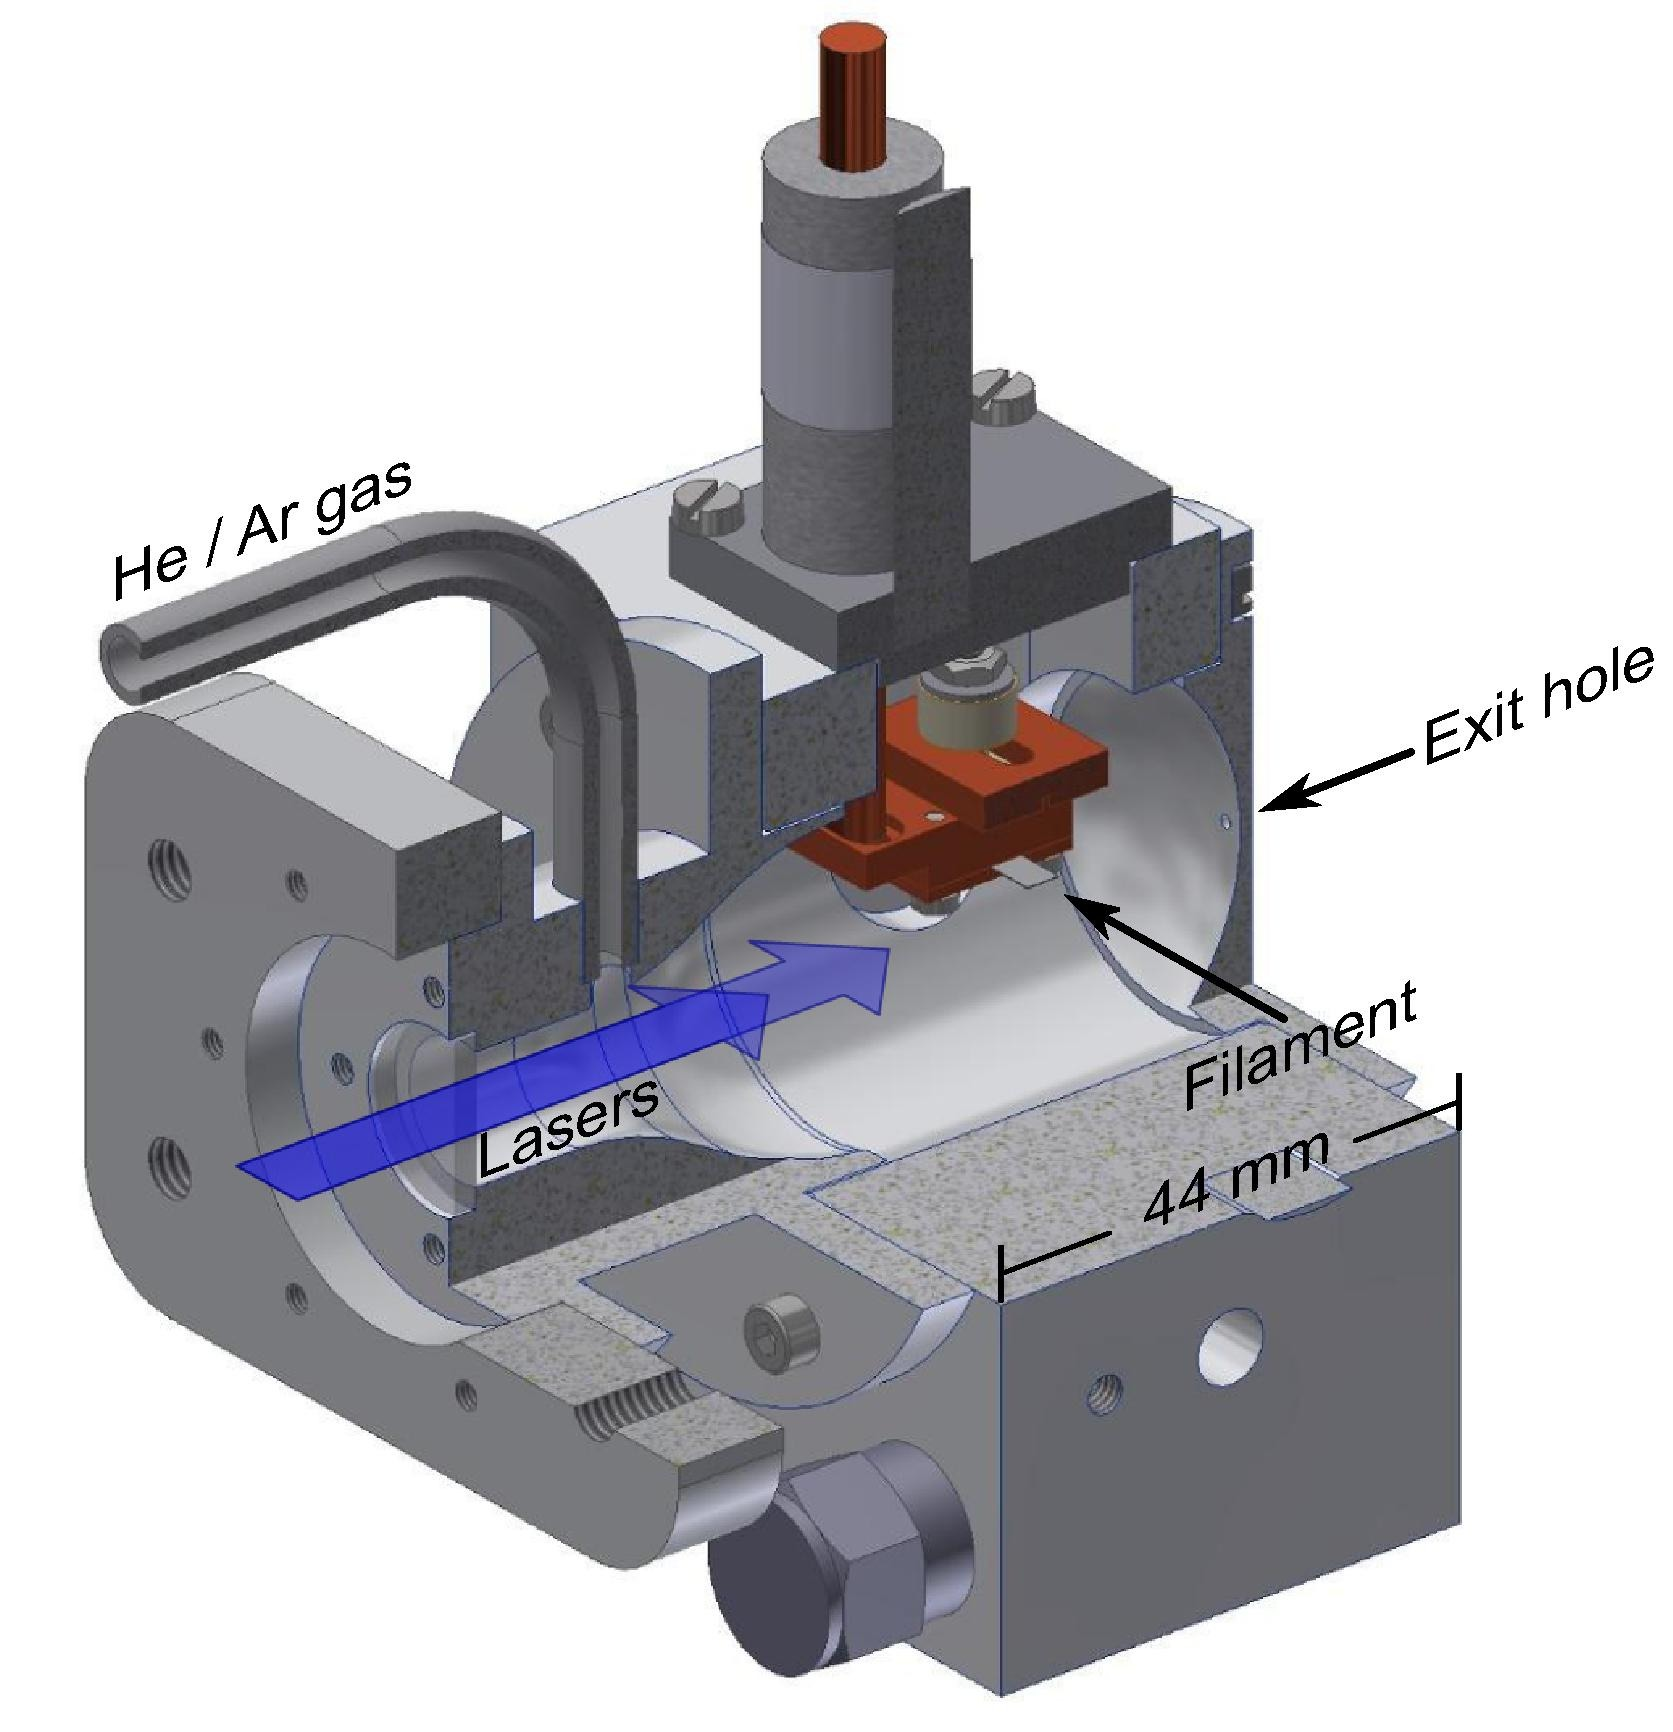
\includegraphics[width=0.8\textwidth]{PuGasCell.jpg}
		\end{textblock*}

		\begin{textblock*}{0.7\paperwidth}(0.32\paperwidth,0.45\paperheight)
			\textbf{Resonance Ionization Spectroscopy and Gas Phase Chemistry}
		\end{textblock*}

		\begin{textblock*}{0.35\paperwidth}(0.62\paperwidth,0.55\paperheight)
			\textbf{Plutonium}
			\begin{itemize}
				\item $^{238-242,244}$Pu on Ta substrate, 1100$^\circ$C
				\item Molecular recombination and collisional de-excitation
			\end{itemize}
		\end{textblock*}
		\begin{textblock*}{0.12\paperwidth}(0.02\paperwidth,0.55\paperheight)
			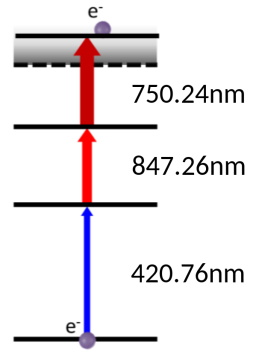
\includegraphics[width=\textwidth]{RIS.png}
		\end{textblock*}
		\begin{textblock*}{0.3\paperwidth}(0.3\paperwidth,0.52\paperheight)
			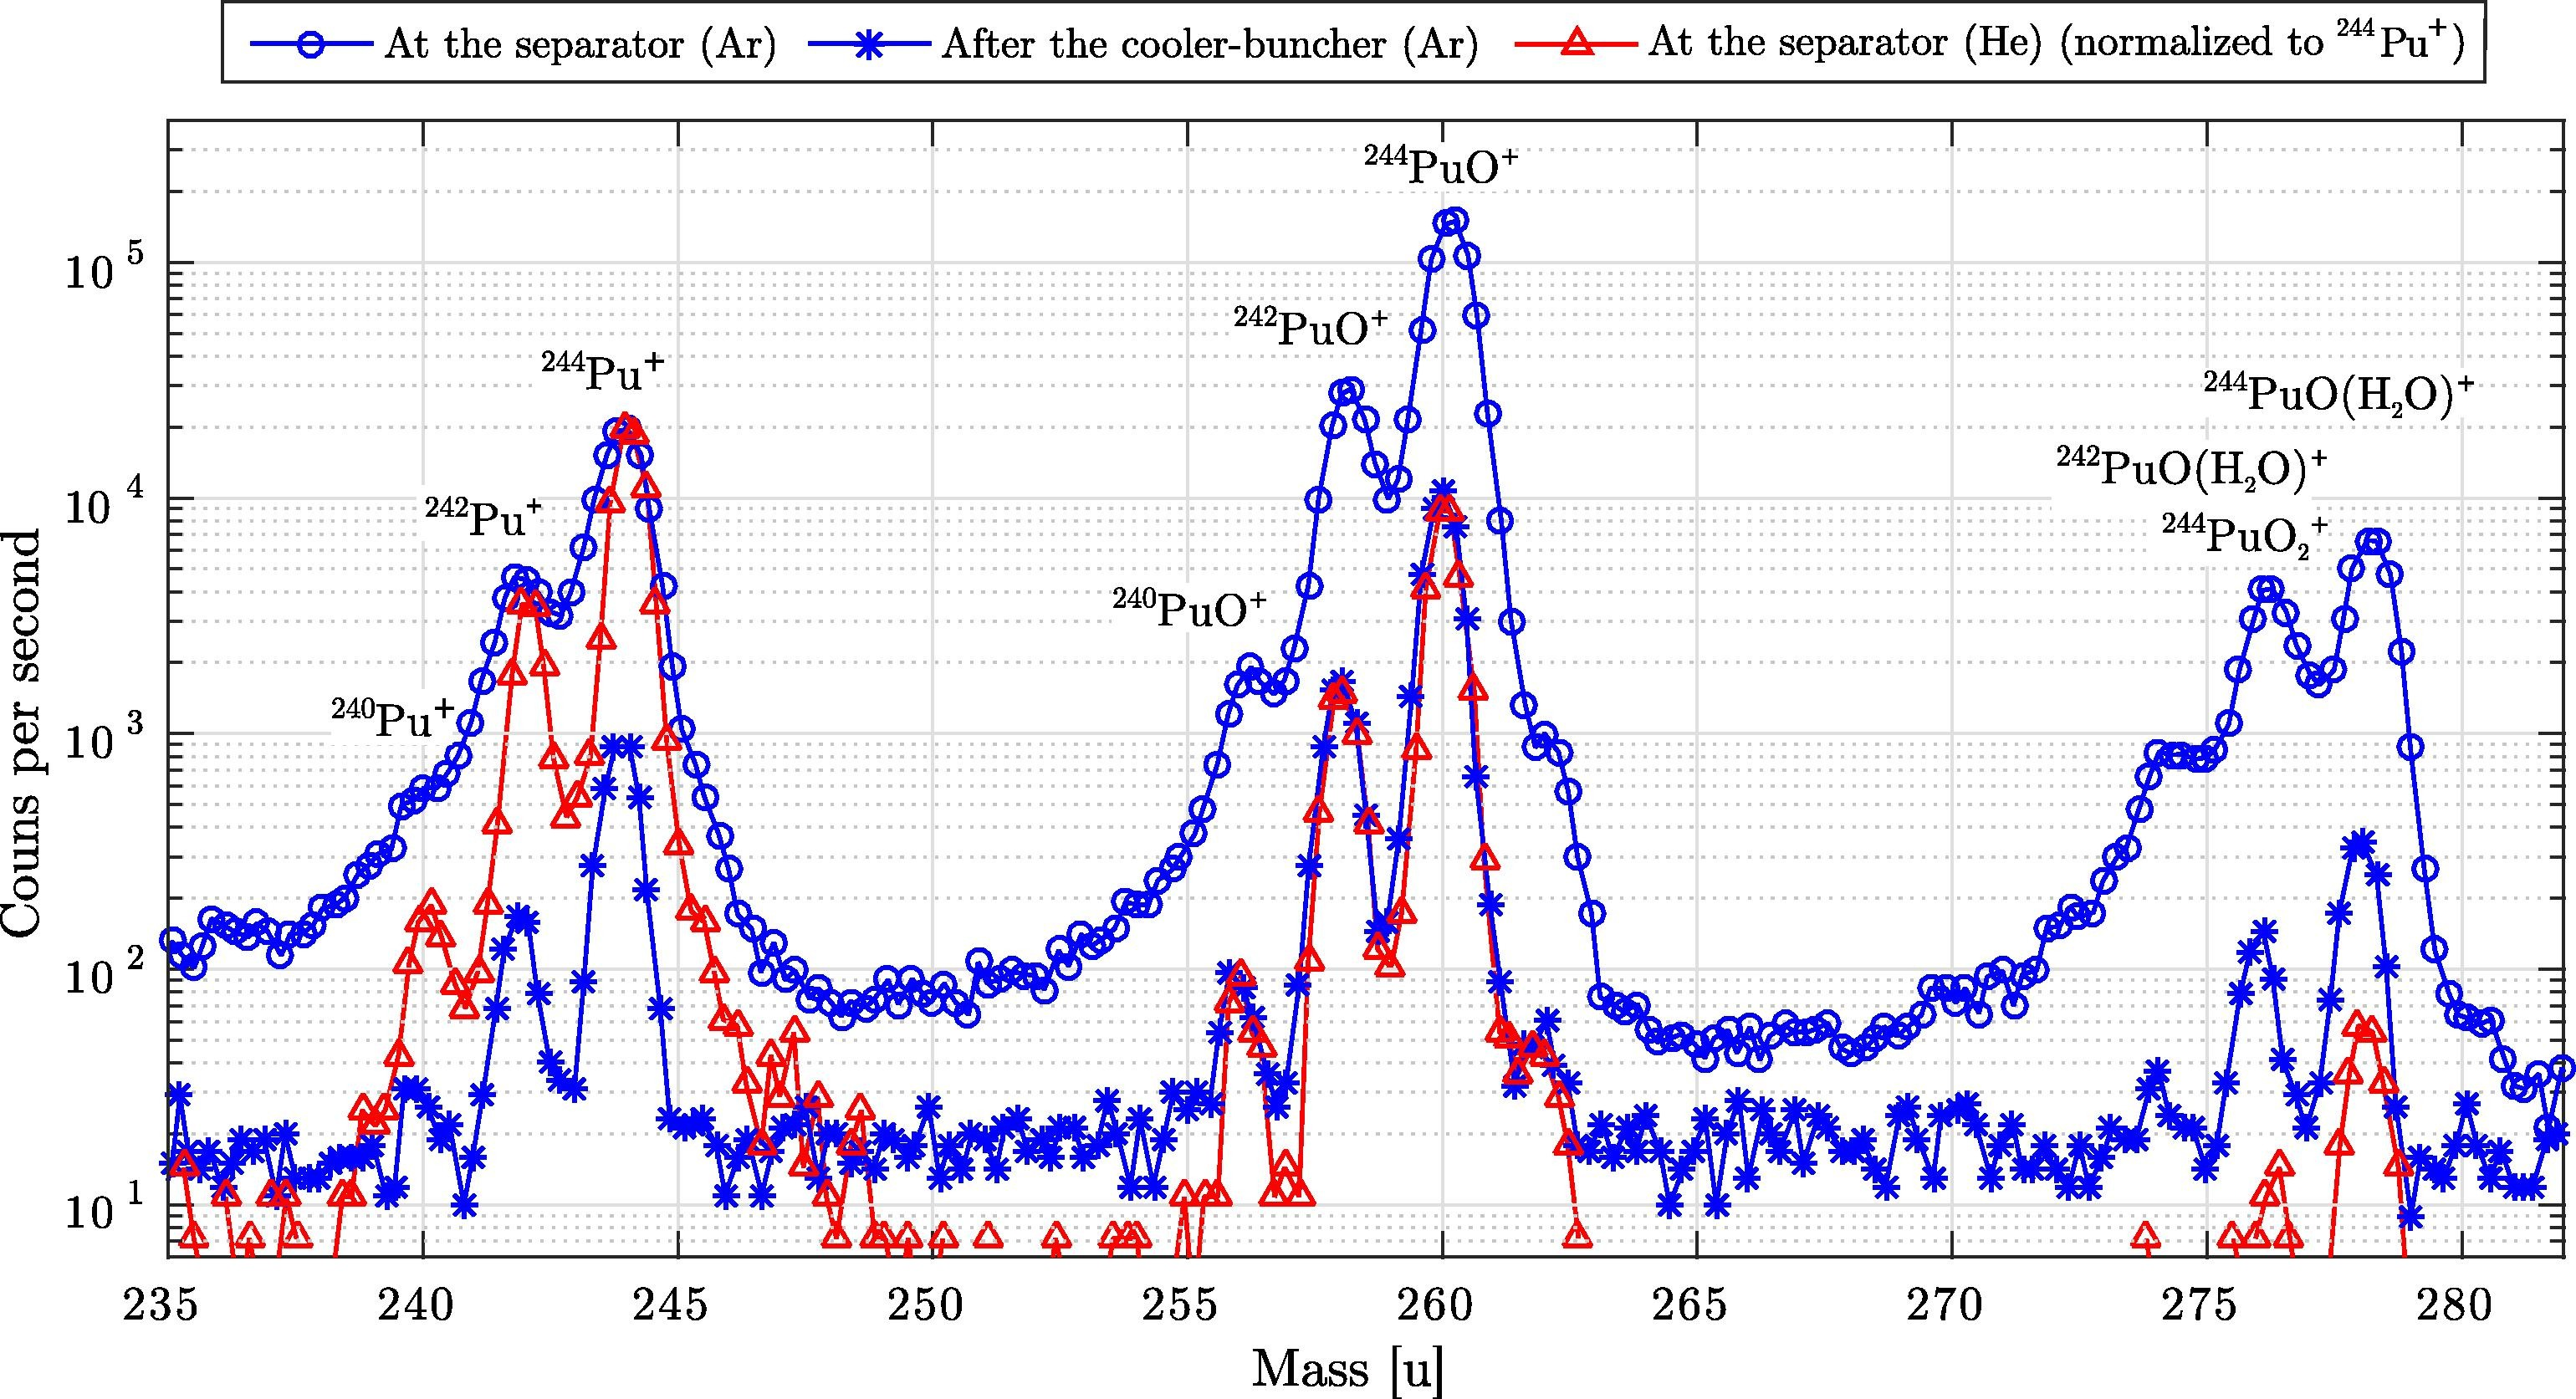
\includegraphics[width=\textwidth]{PuRIS.jpg}
		\end{textblock*}
		\begin{textblock*}{0.1\paperwidth}(0.61\paperwidth,0.8\paperheight)
			\footnote{I. Pohjalainen, I.M. et al., NIMB 376 (2016) 233}
		\end{textblock*}
	}
	\only<2>{
		\begin{textblock*}{0.185\paperwidth}(0.12\paperwidth,0.17\paperheight)
			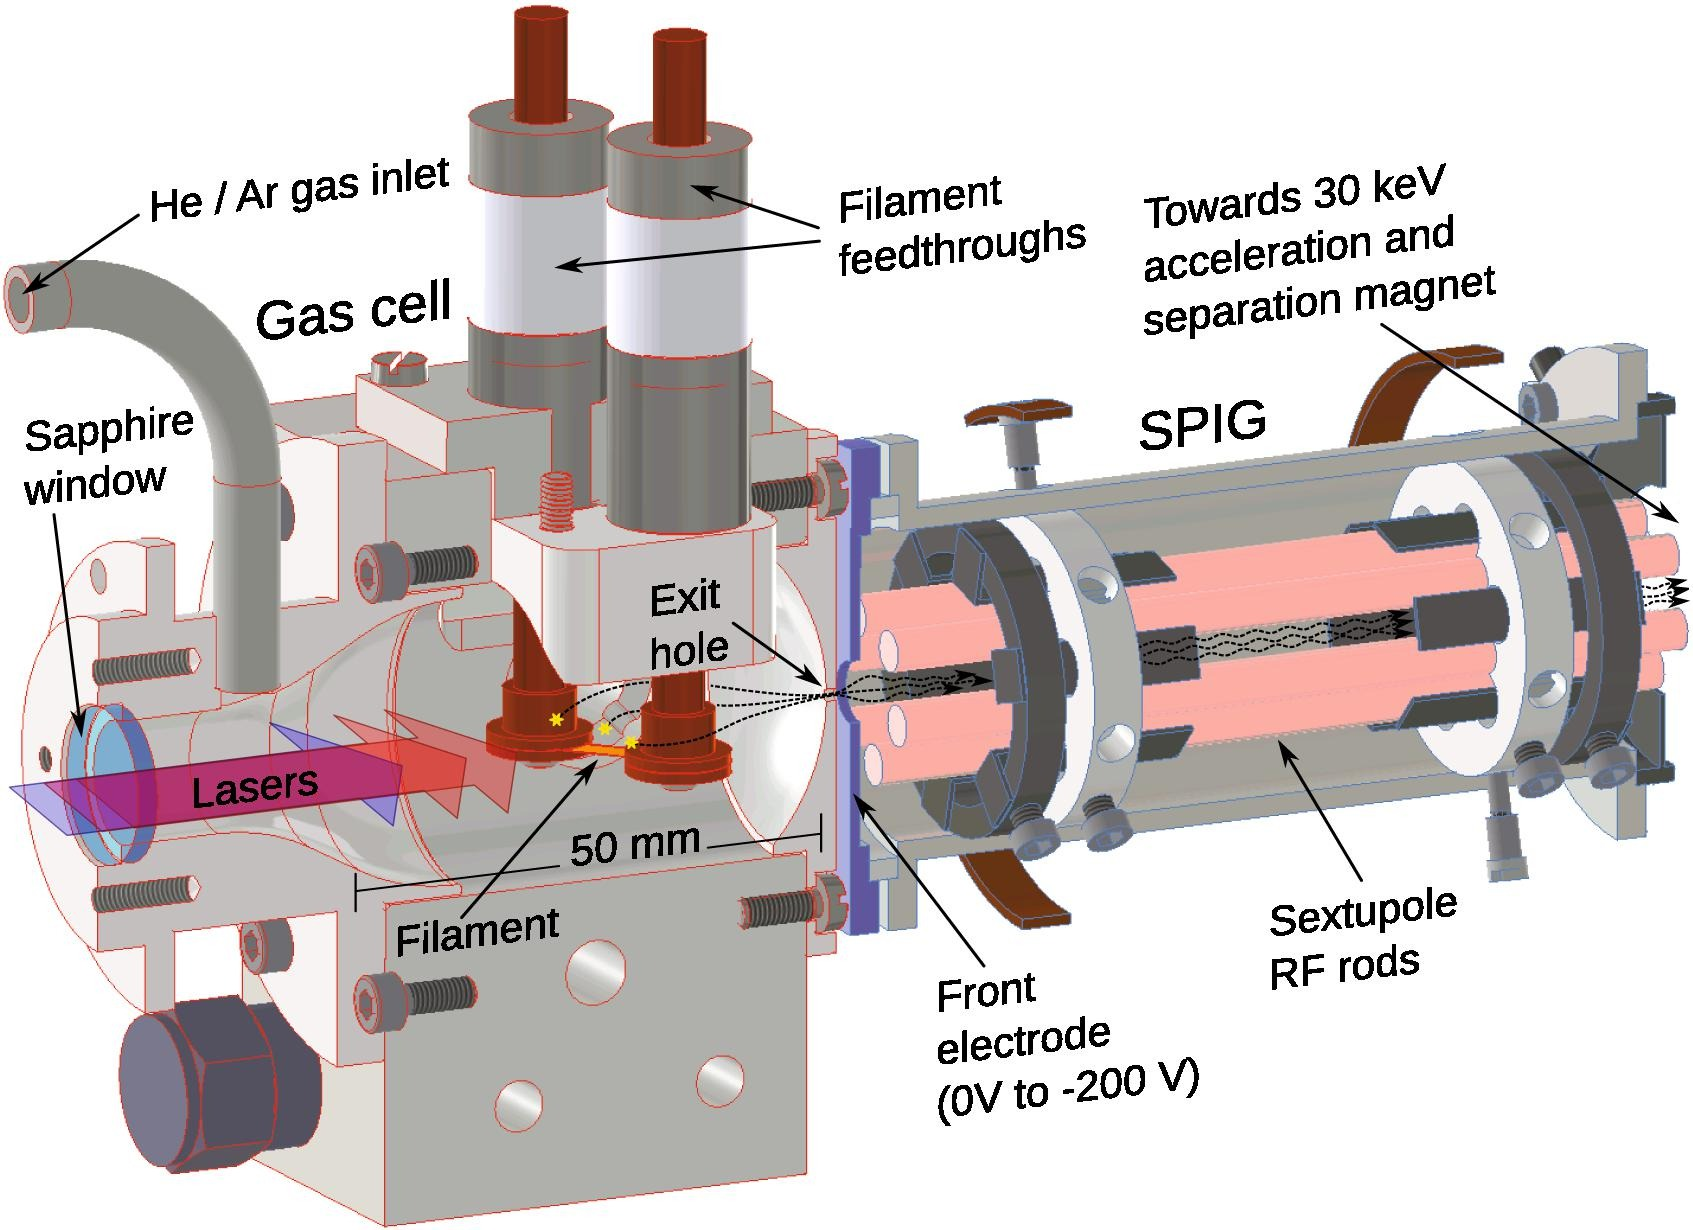
\includegraphics[width=\textwidth]{GasCell.jpg}
		\end{textblock*}
		\begin{textblock*}{0.1\paperwidth}(0.28\paperwidth,0.42\paperheight)
			\footnote{I. Pohjalainen, NIM B ,484 (2020) 59-70}
		\end{textblock*}

		\begin{textblock*}{0.7\paperwidth}(0.32\paperwidth,0.45\paperheight)
			\textbf{Resonance Ionization Spectroscopy and Gas Phase Chemistry}
		\end{textblock*}

		\begin{textblock*}{0.35\paperwidth}(0.62\paperwidth,0.55\paperheight)
			\textbf{Thorium}
			\begin{itemize}
				\item ---
			\end{itemize}
		\end{textblock*}
		\begin{textblock*}{0.15\paperwidth}(0.02\paperwidth,0.57\paperheight)
			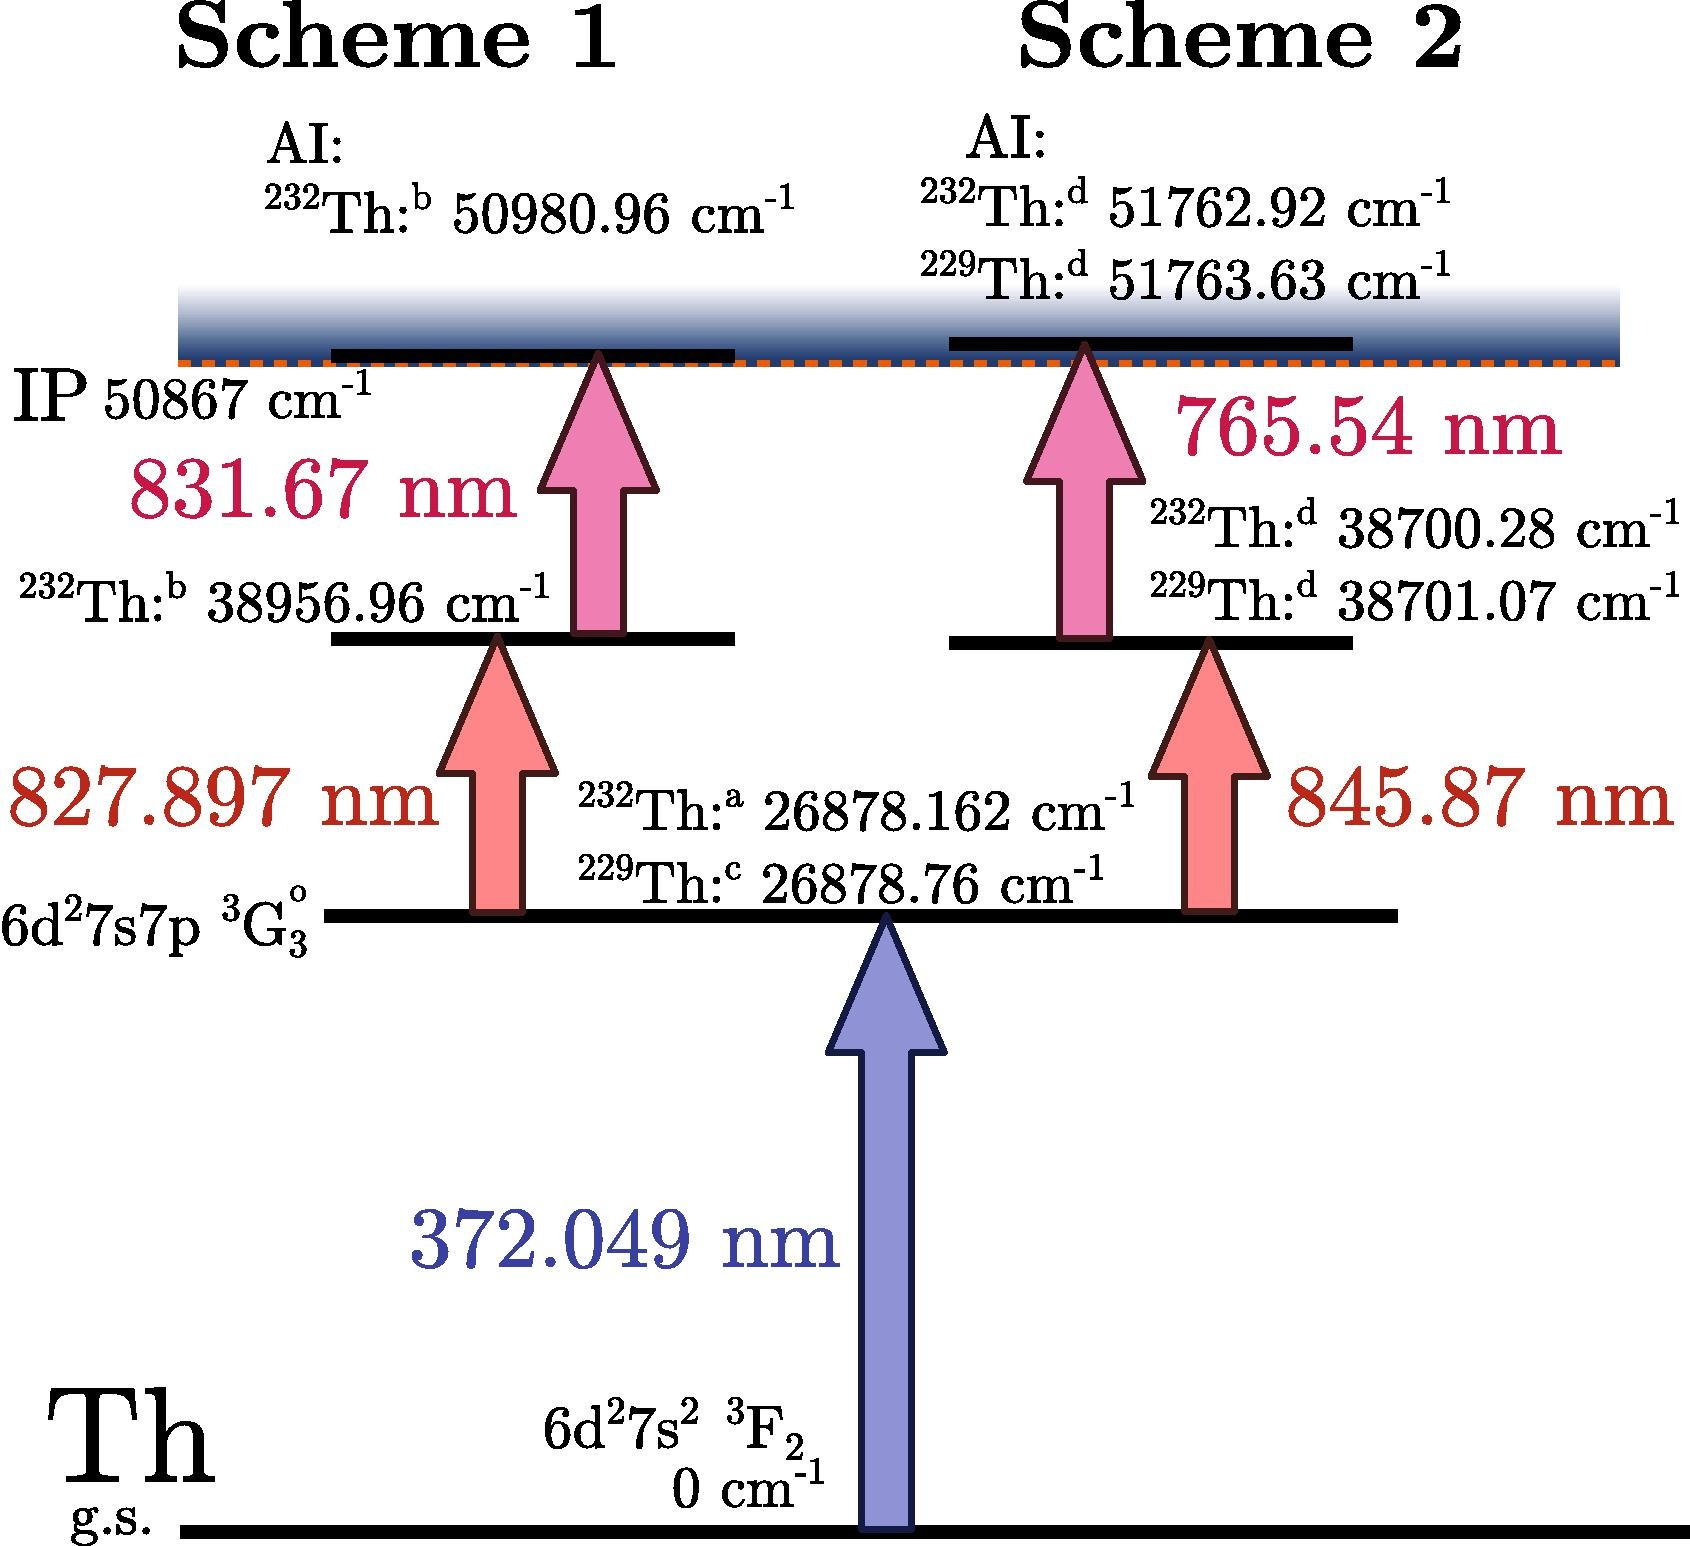
\includegraphics[width=\textwidth]{ThScheme.jpg}
		\end{textblock*}
		\begin{textblock*}{0.3\paperwidth}(0.3\paperwidth,0.52\paperheight)
			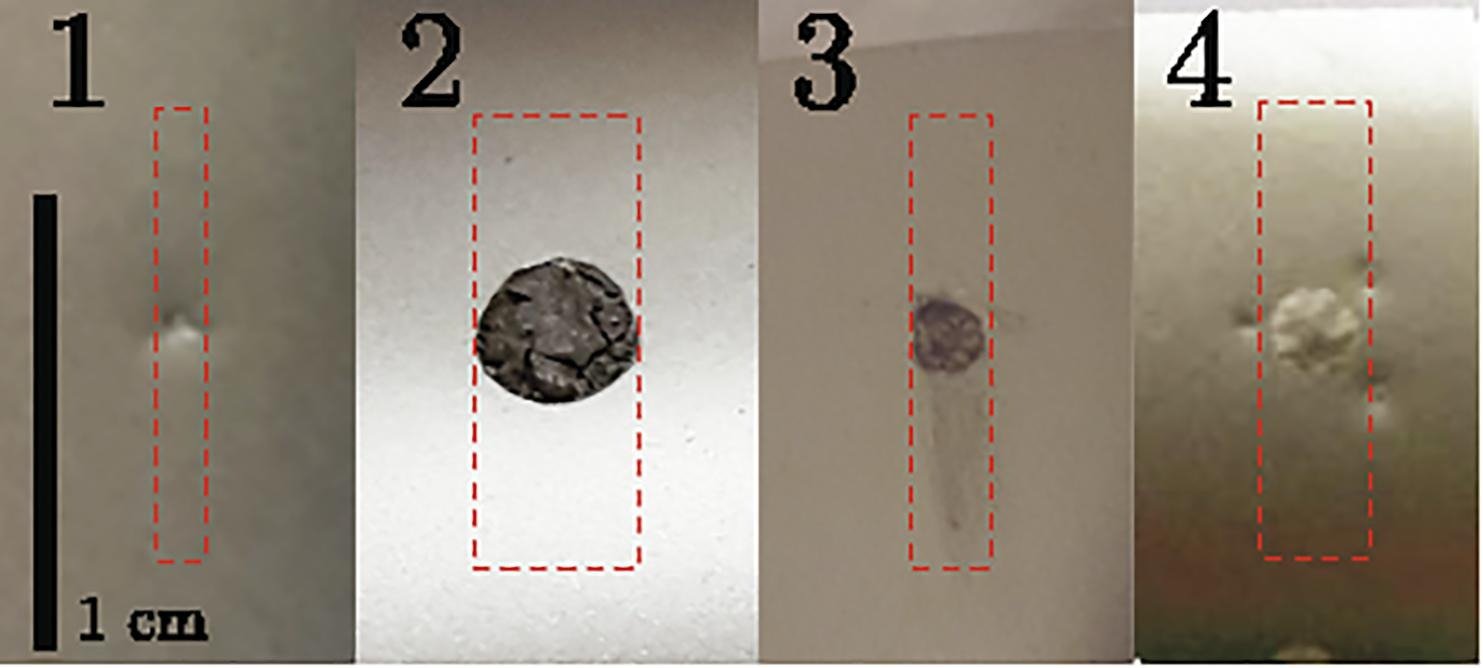
\includegraphics[width=\textwidth]{ThRIS.jpg}
		\end{textblock*}
	}
	\only<3>{
		\begin{textblock*}{0.185\paperwidth}(0.12\paperwidth,0.17\paperheight)
			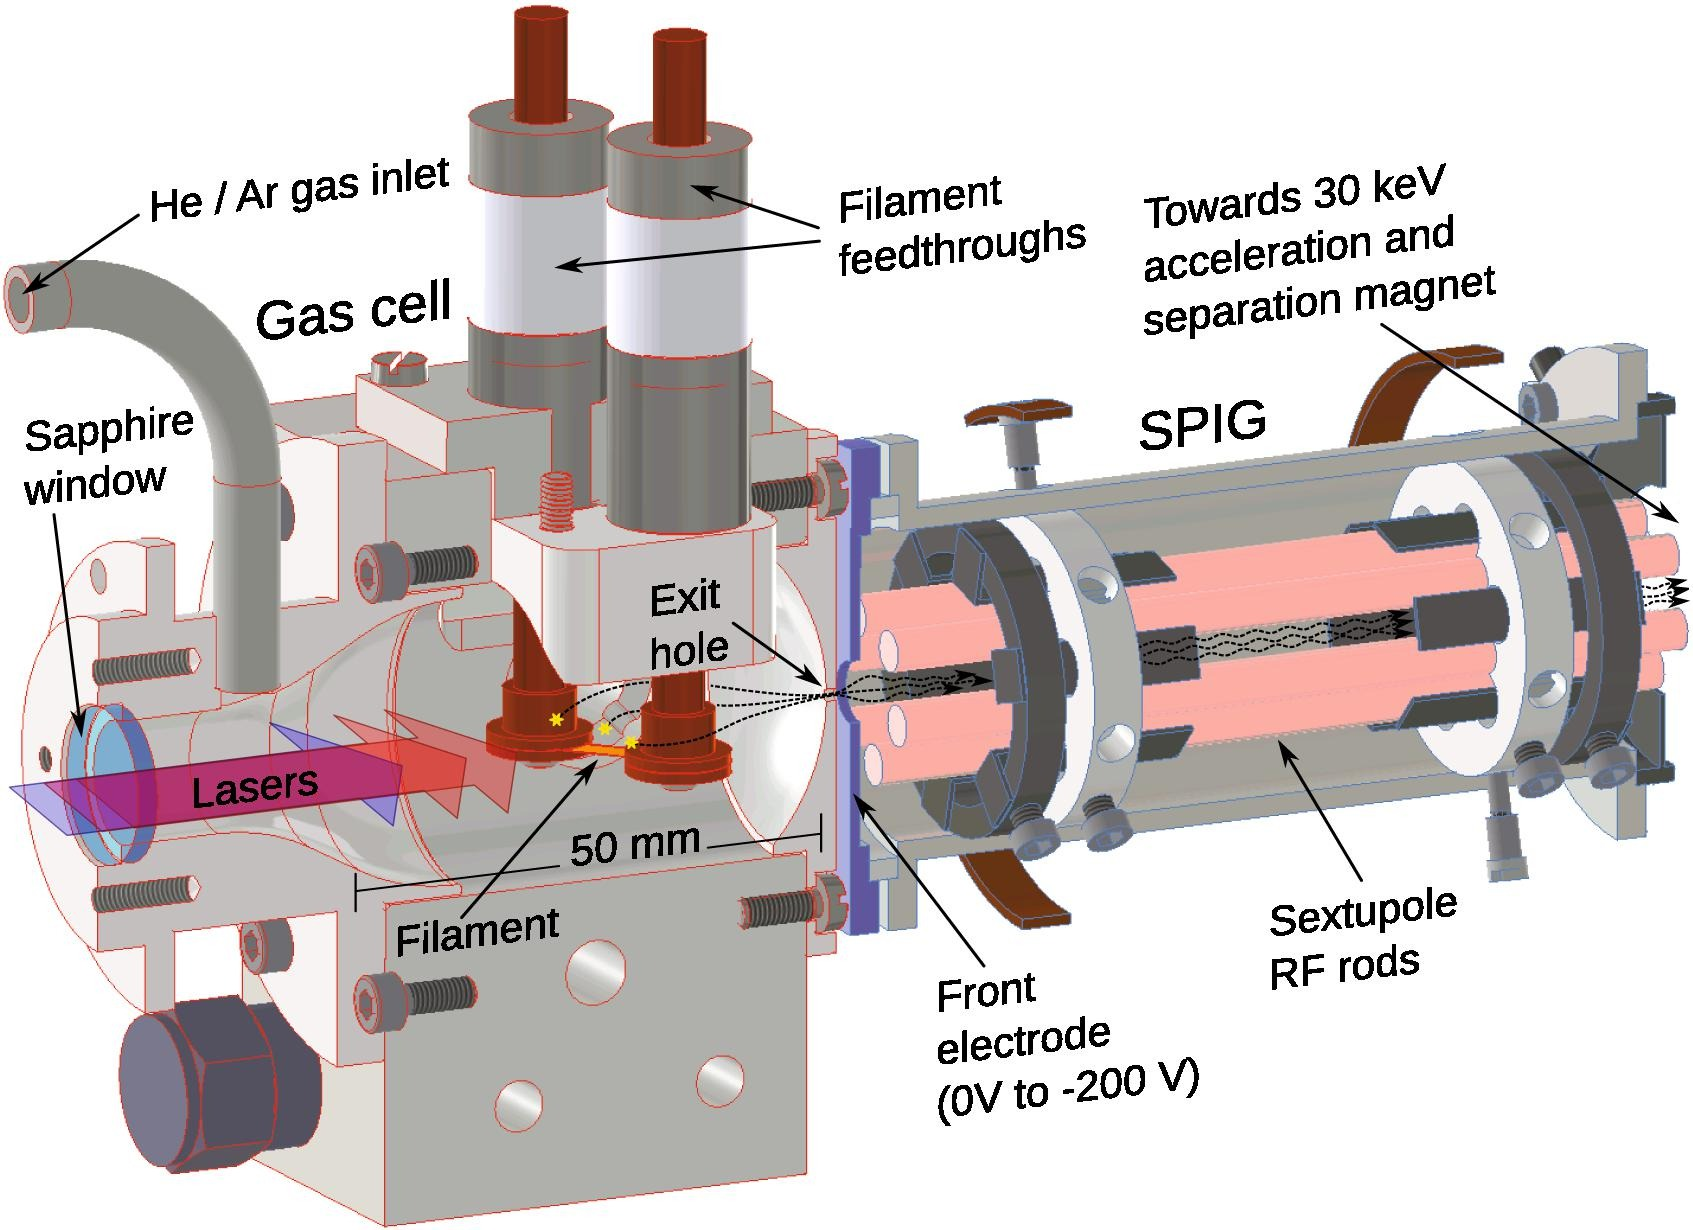
\includegraphics[width=\textwidth]{GasCell.jpg}
		\end{textblock*}
		\begin{textblock*}{0.1\paperwidth}(0.28\paperwidth,0.42\paperheight)
			\footnote{I. Pohjalainen, NIM B ,484 (2020) 59-70}
		\end{textblock*}

		\begin{textblock*}{0.7\paperwidth}(0.4\paperwidth,0.45\paperheight)
			\textbf{Use of $^{233}$U as $^{229}$Th alpha recoil source}
		\end{textblock*}

		\begin{textblock*}{0.5\paperwidth}(0.62\paperwidth,0.5\paperheight)
			\textbf{MLU}
			\begin{itemize}
				\item UF$_4$, 240kBq, Evaporated on Al
				\item 420 nm
			\end{itemize}
			\textbf{JYU}
			\begin{itemize}
				\item U, 2.3MBq, Electroplated
				\item 12 nm
			\end{itemize}
		\end{textblock*}
		\begin{textblock*}{0.15\paperwidth}(0.02\paperwidth,0.55\paperheight)
			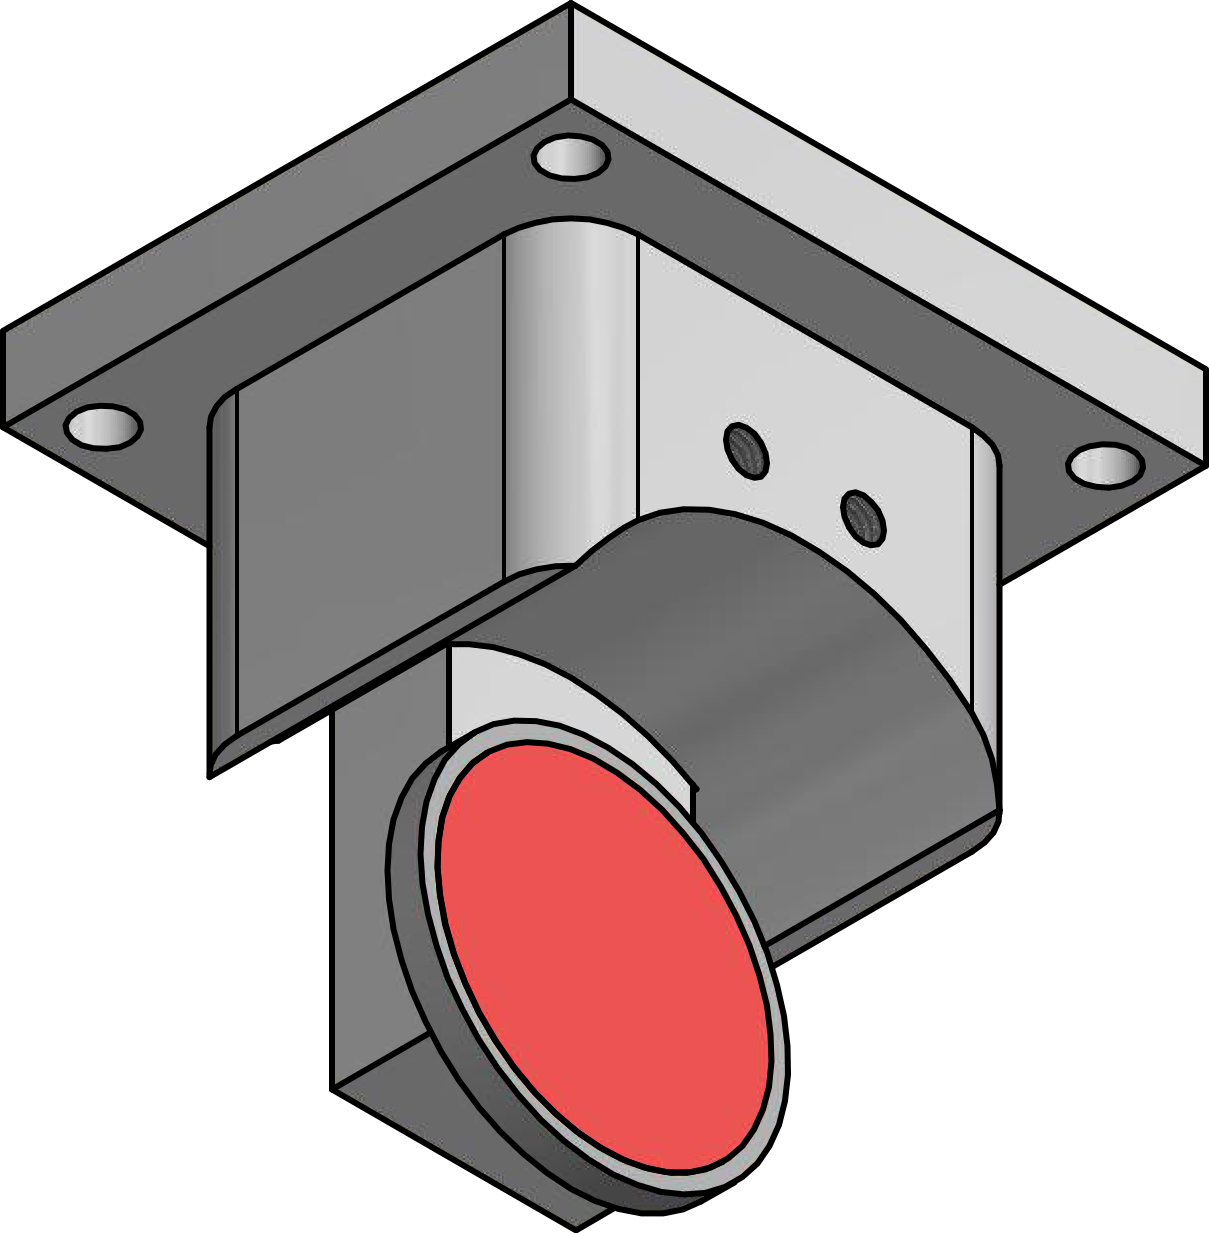
\includegraphics[width=\textwidth]{U233SRC.png}
		\end{textblock*}
		\begin{textblock*}{0.2\paperwidth}(0.3\paperwidth,0.5\paperheight)
			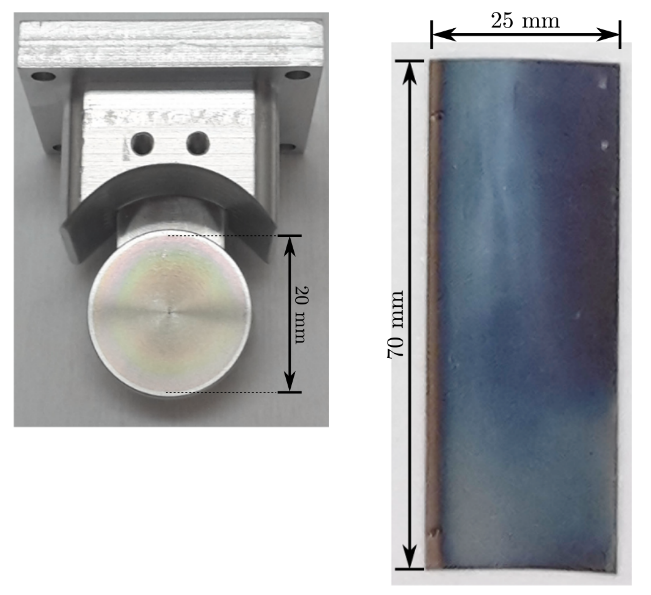
\includegraphics[width=\textwidth]{sources_comparison.png}
		\end{textblock*}
		\begin{textblock*}{0.07\paperwidth}(0.3\paperwidth,0.75\paperheight)
			\footnote{I. Pohjalainen, NIM B ,463 (2020) 441-448}
		\end{textblock*}
		\begin{textblock*}{0.12\paperwidth}(0.48\paperwidth,0.5\paperheight)
			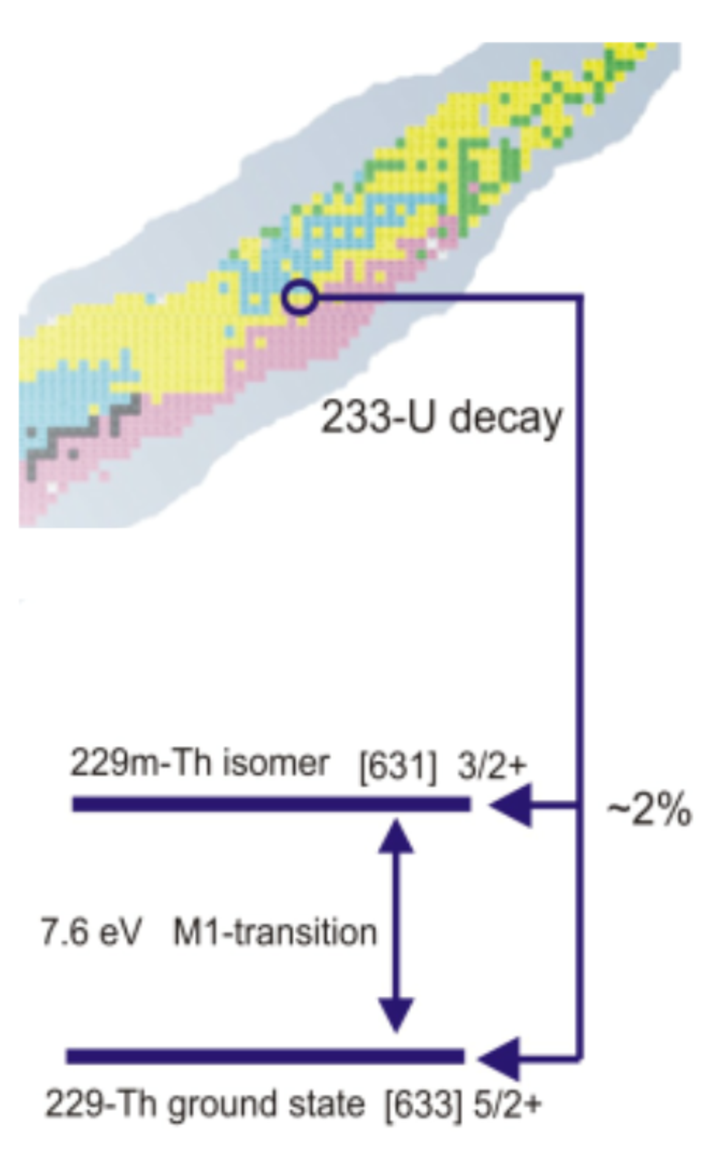
\includegraphics[width=\textwidth]{233Udecay.pdf}
		\end{textblock*}
	}
	% 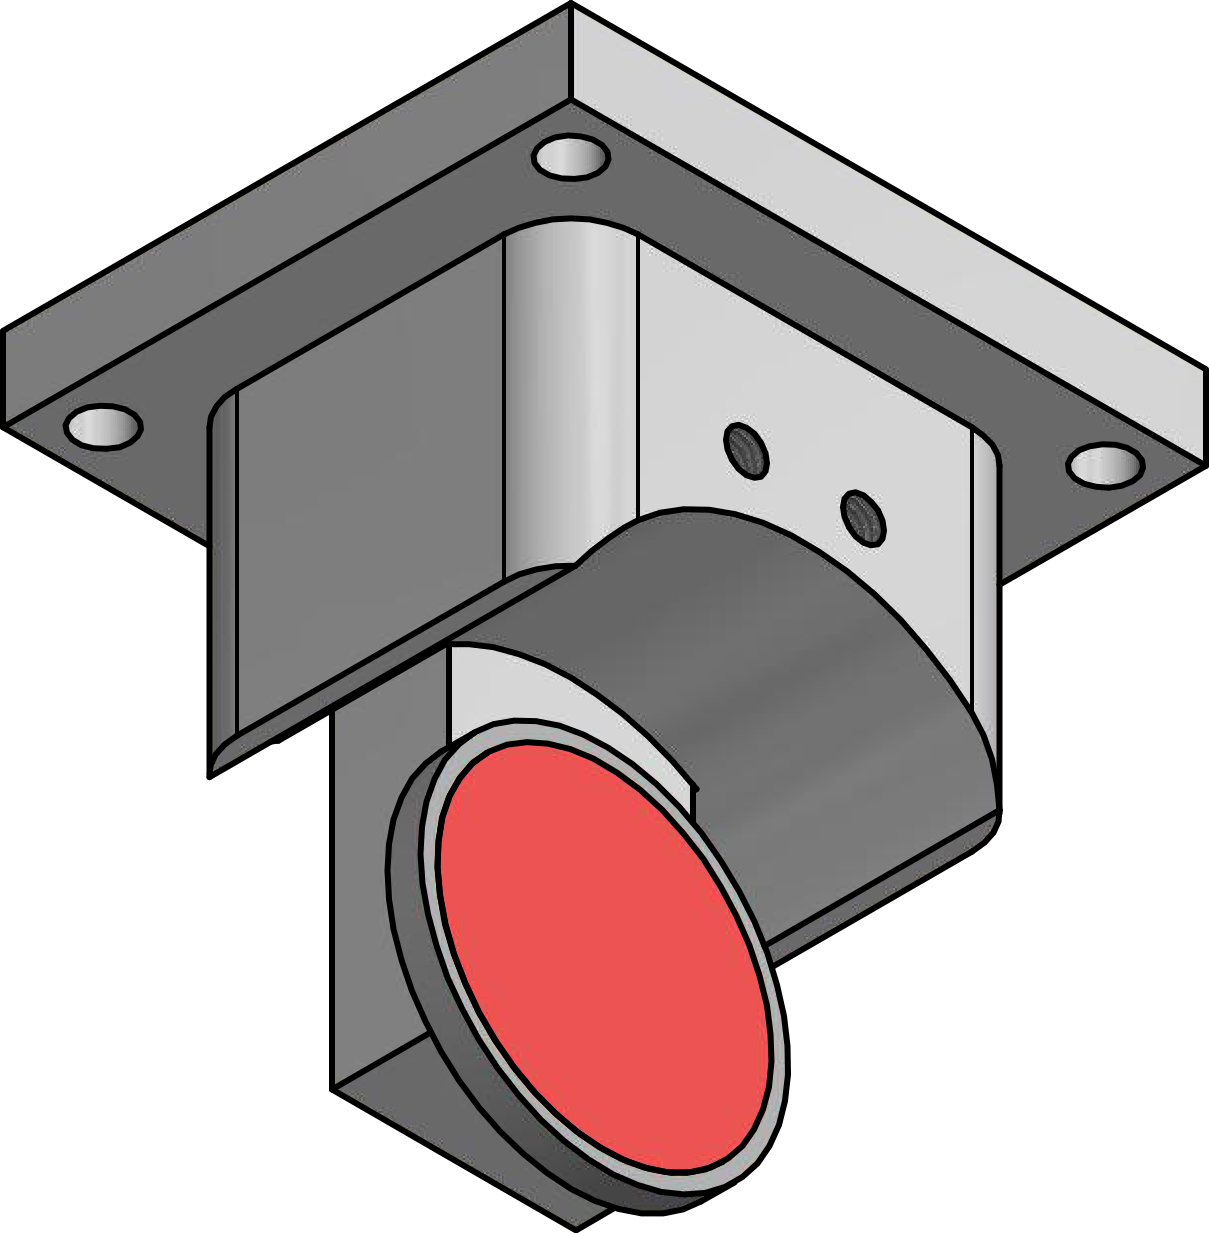
\includegraphics[width = 0.1\textwidth]{U233SRC.png}
\end{frame}

\begin{frame}{Online Production}
	\begin{textblock*}{0.8\paperwidth}(0.01\paperwidth,0.1\paperheight)
		% \only<1->{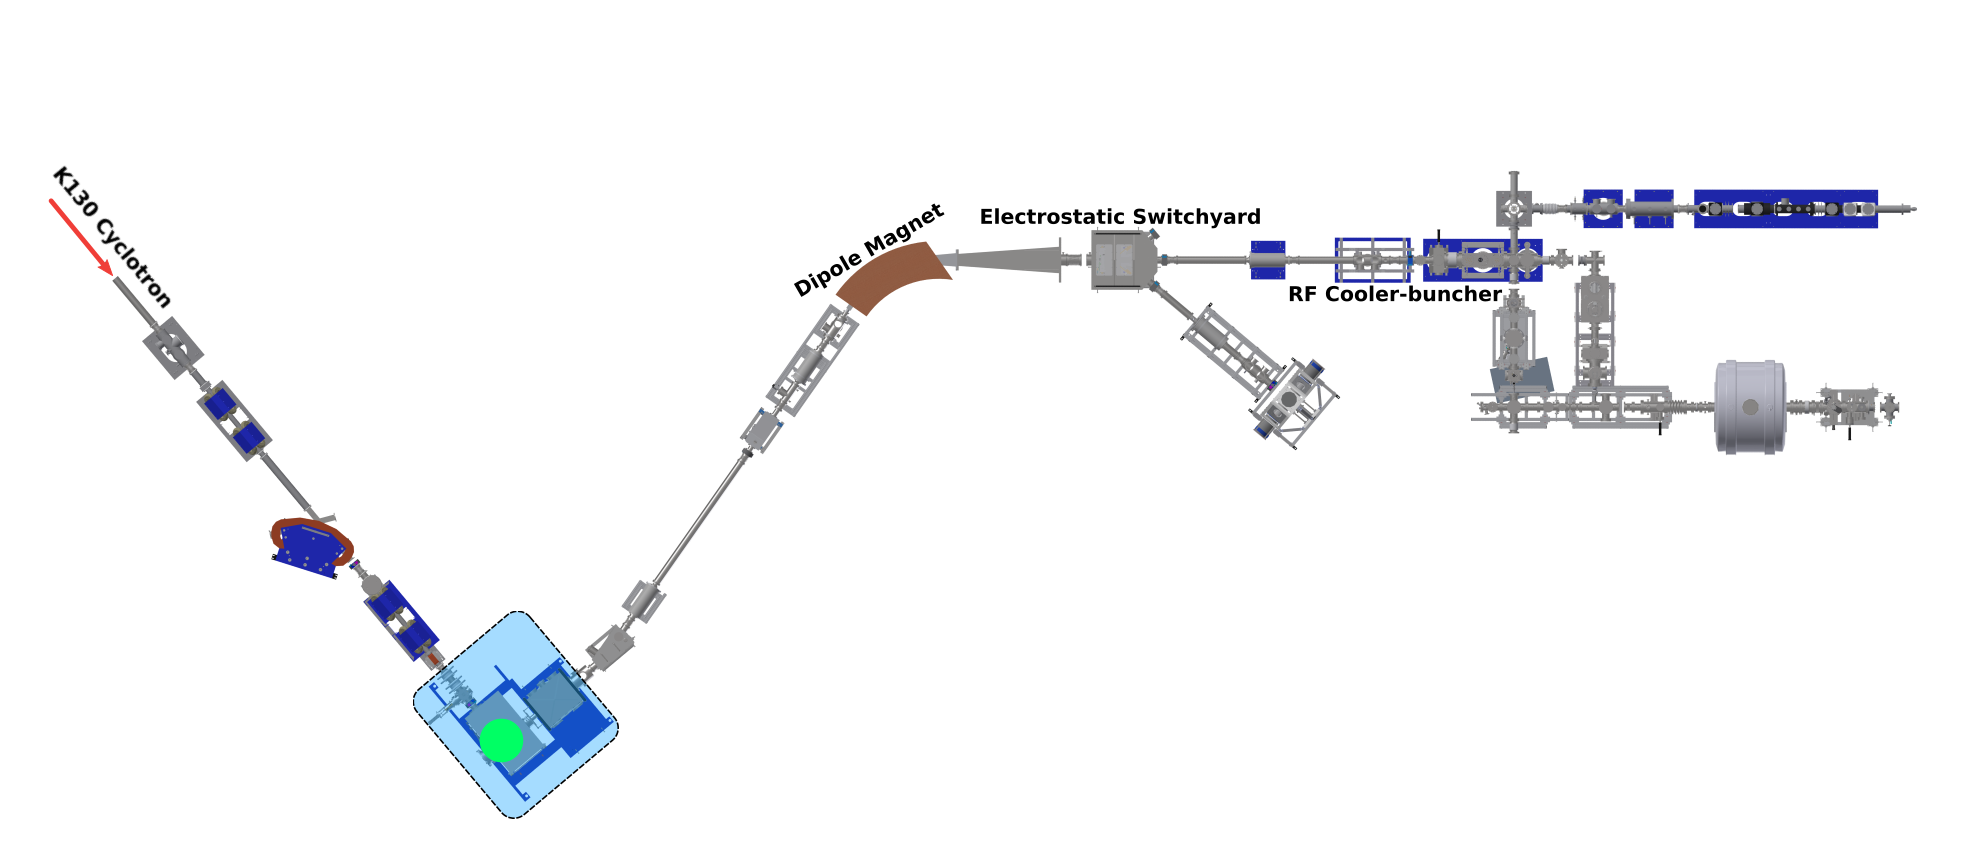
\includegraphics[width=\textwidth]{Igisol_scheme_TG.png}}%
		\only<1->{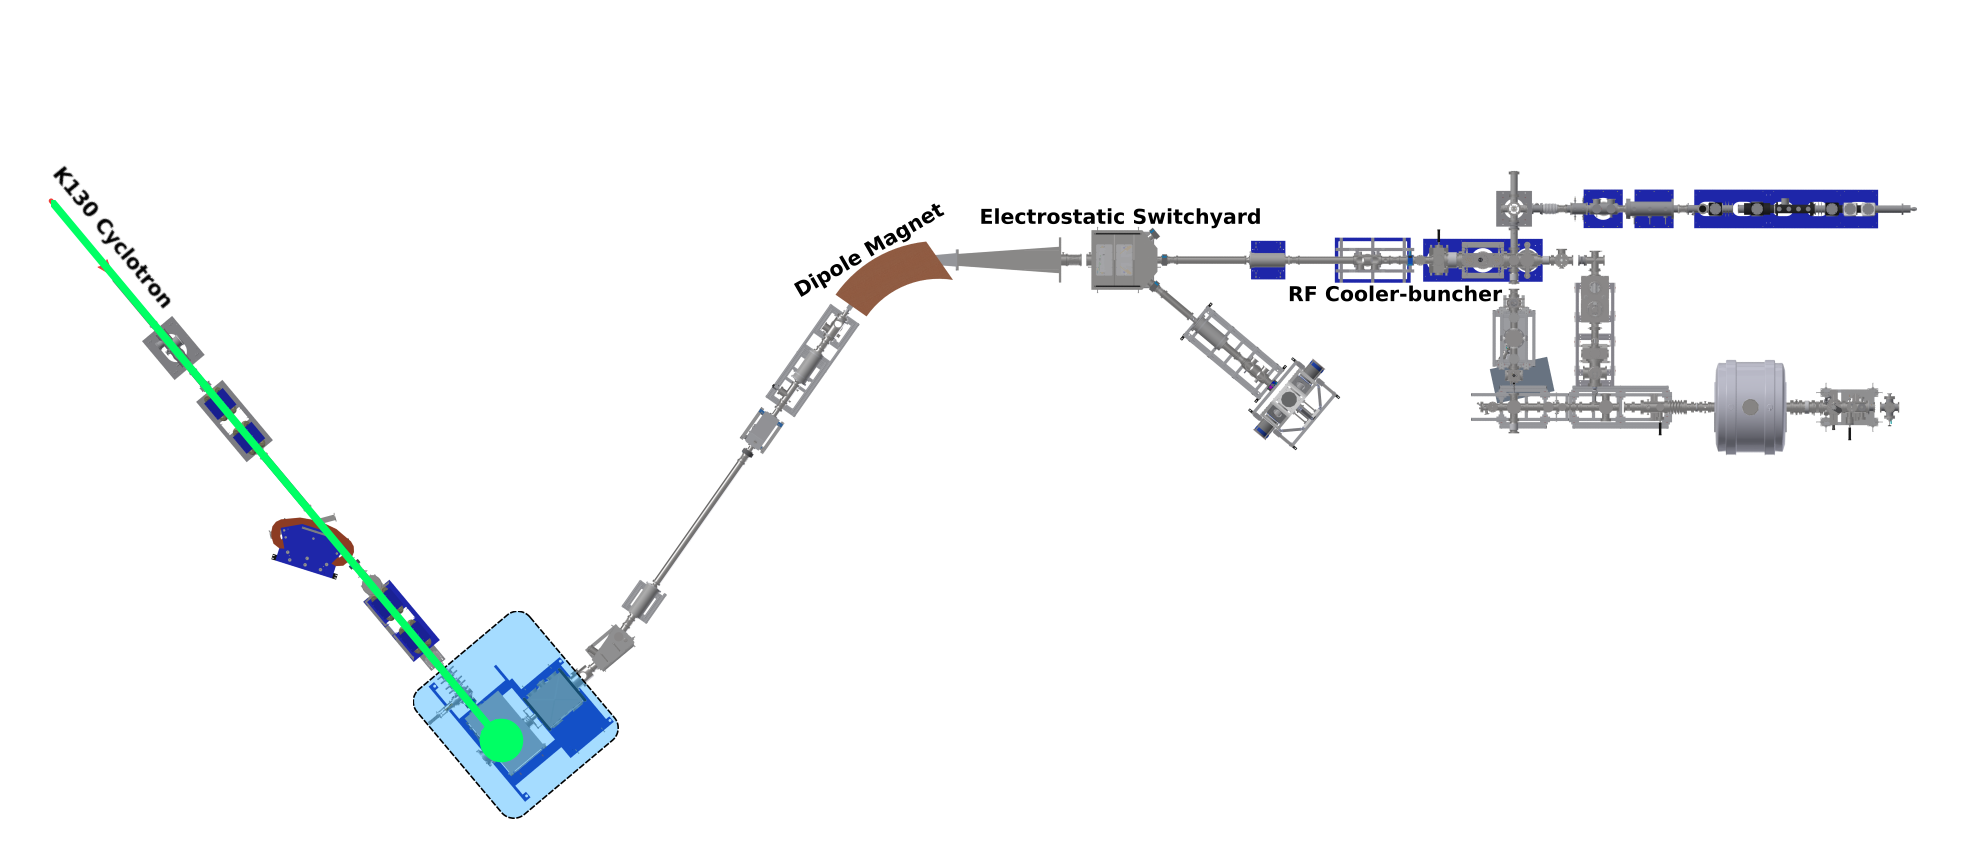
\includegraphics[width=\textwidth]{Igisol_scheme_TG_online.png}}%
		% \only<4>{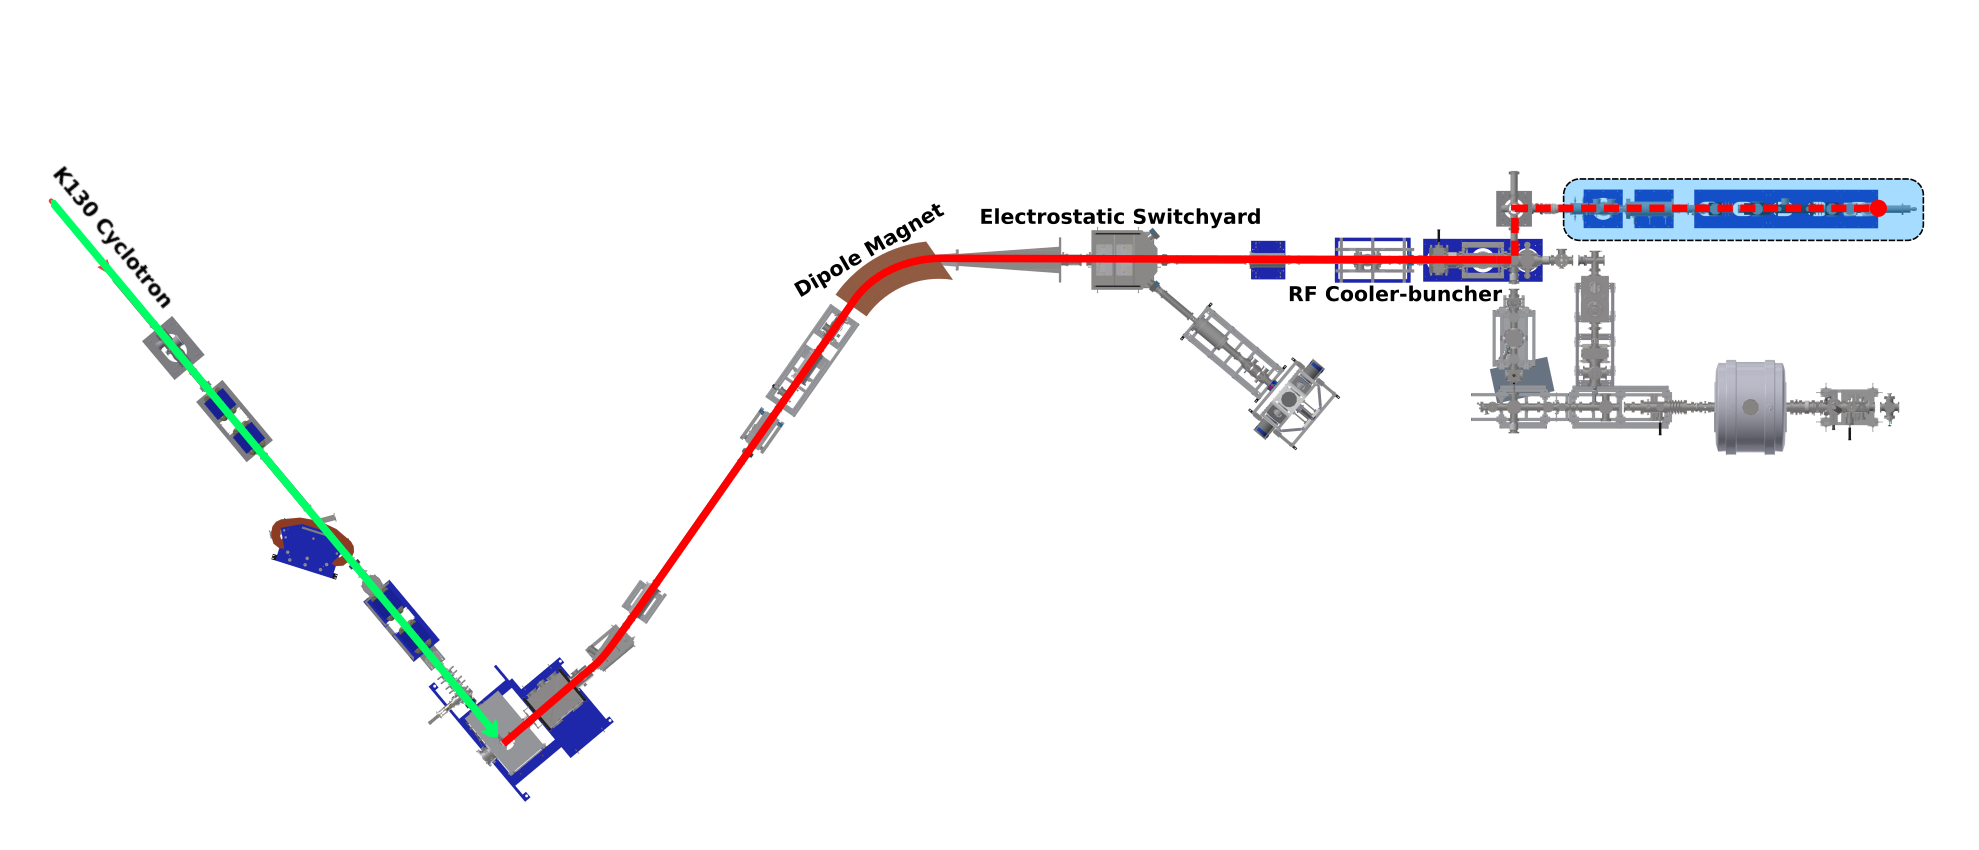
\includegraphics[width=\textwidth]{Igisol_scheme_CLS.png}}%
		% \only<5>{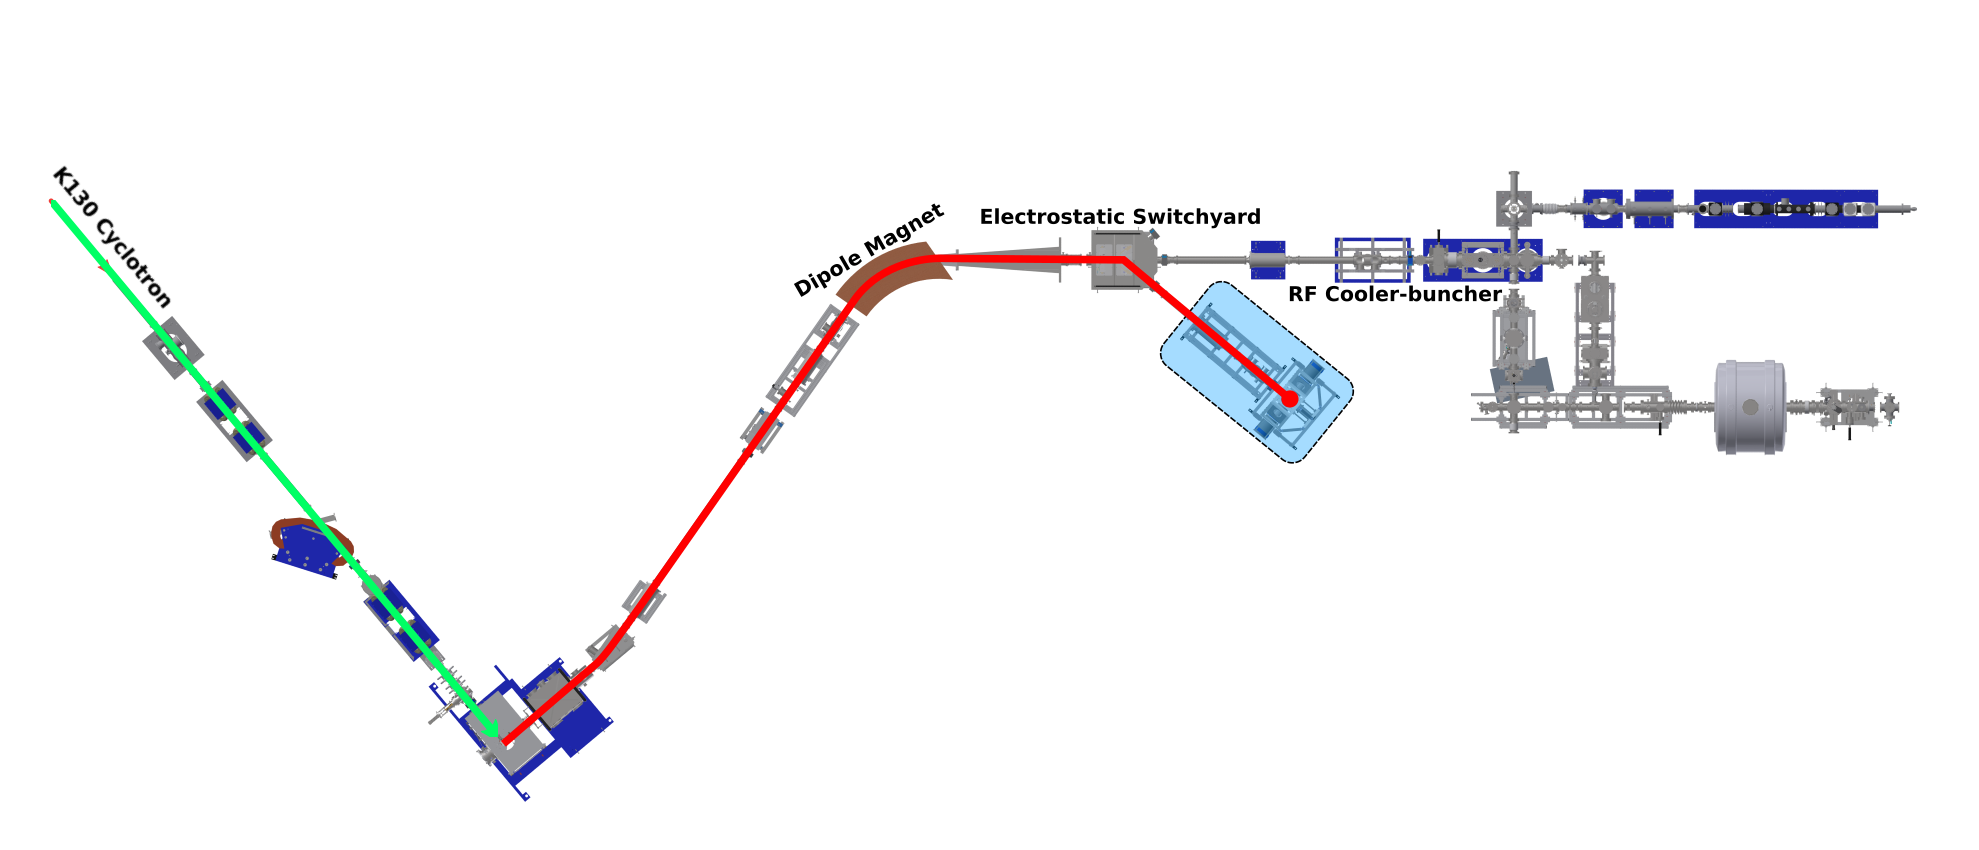
\includegraphics[width=\textwidth]{Igisol_scheme_Spec.png}}%
		% \only<6>{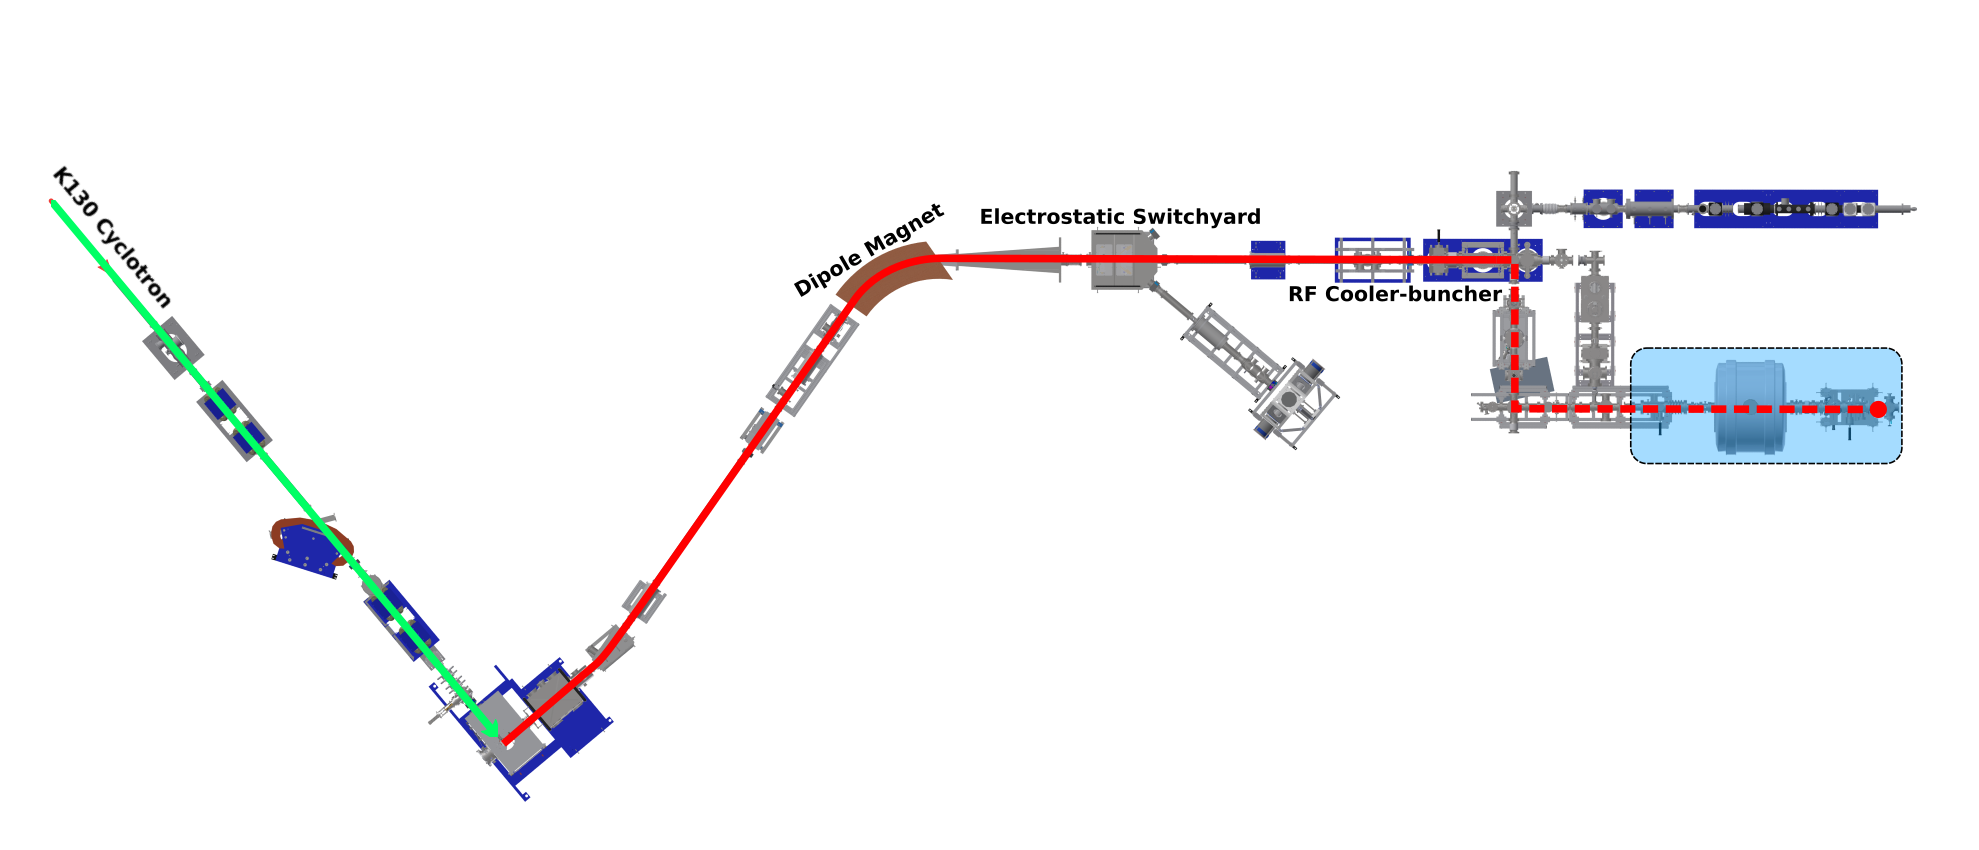
\includegraphics[width=\textwidth]{Igisol_scheme_Penn.png}}%
	\end{textblock*}
	\only<1>{
		\begin{textblock*}{0.19\paperwidth}(0.14\paperwidth,0.2\paperheight)
			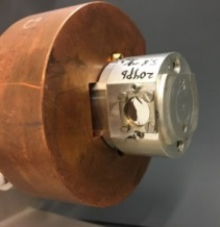
\includegraphics[width=0.8\textwidth]{LIONGUIDE.png}
		\end{textblock*}

		\begin{textblock*}{0.7\paperwidth}(0.32\paperwidth,0.45\paperheight)
			\textbf{Proton-Induced Fusion-evaporation reactions}
		\end{textblock*}

		\begin{textblock*}{0.5\paperwidth}(0.45\paperwidth,0.5\paperheight)
			\begin{itemize}
				\item Production of neutron deficient actinides
				\item Extraction times can be < 1ms 
			\end{itemize}
		\end{textblock*}
		\begin{textblock*}{0.15\paperwidth}(0.005\paperwidth,0.55\paperheight)
			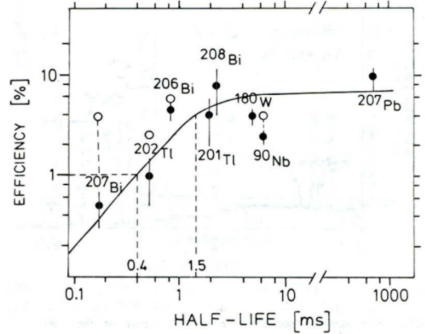
\includegraphics[width=\textwidth]{OldEfficiency.png}
		\end{textblock*}
		\begin{textblock*}{0.3\paperwidth}(0.16\paperwidth,0.49\paperheight)
			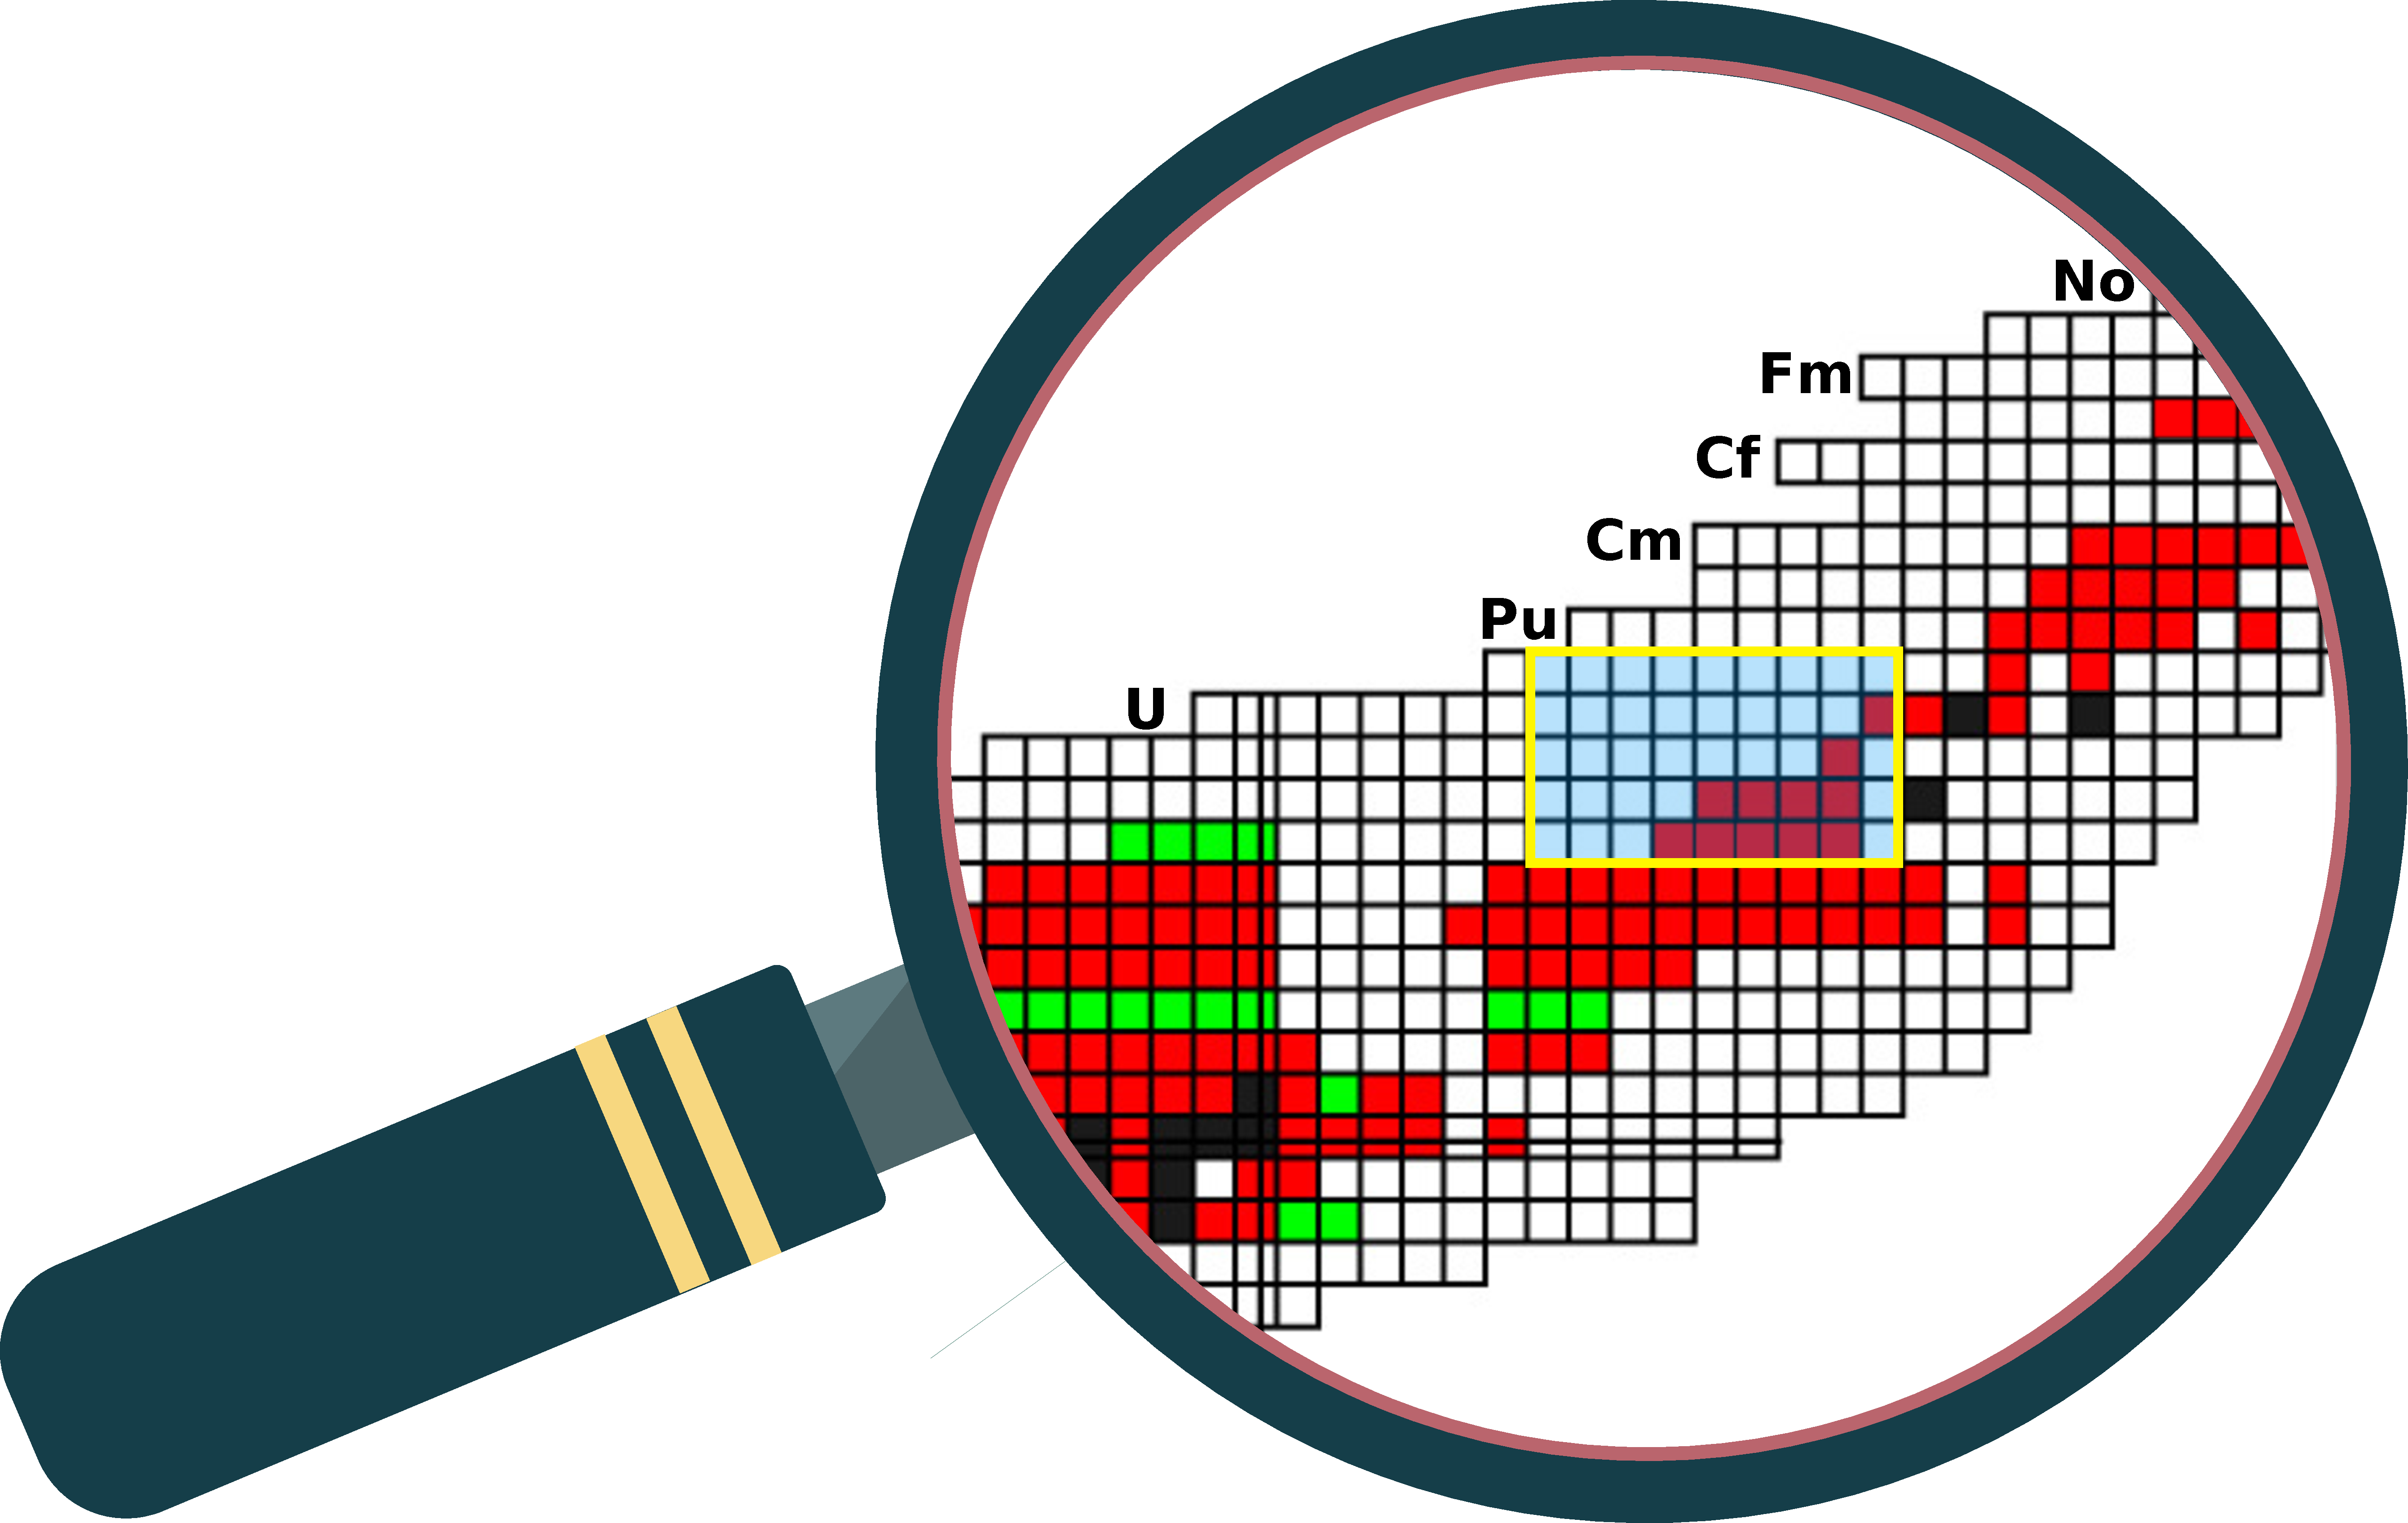
\includegraphics[width=\textwidth]{AChart_zoom.pdf}
		\end{textblock*}
		\begin{textblock*}{0.2\paperwidth}(0.47\paperwidth,0.64\paperheight)
			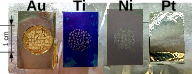
\includegraphics[width=\textwidth]{DODtarget.png}
		\end{textblock*}
		\begin{textblock*}{0.3\paperwidth}(0.68\paperwidth,0.64\paperheight)
			\textbf{DoD Target}
			\begin{itemize}
				\item Good target durability
				\item Stability of the production yield
			\end{itemize}
		\end{textblock*}
		\begin{textblock*}{0.1\paperwidth}(0.68\paperwidth,0.75\paperheight)
			\footnote{R. Haas et al., NIMA 874 (2017) 43}
		\end{textblock*}
		\begin{textblock*}{0.1\paperwidth}(0.01\paperwidth,0.75\paperheight)
			\footnote{J. Ärje, J. Äystö et al., Phys. Rev. Lett. 54 (1985) 99}
		\end{textblock*}
	}
	
\end{frame}


\begin{frame}{Collinear Laser Spectroscopy}
	\begin{textblock*}{0.8\paperwidth}(0.01\paperwidth,0.1\paperheight)
		% \only<1->{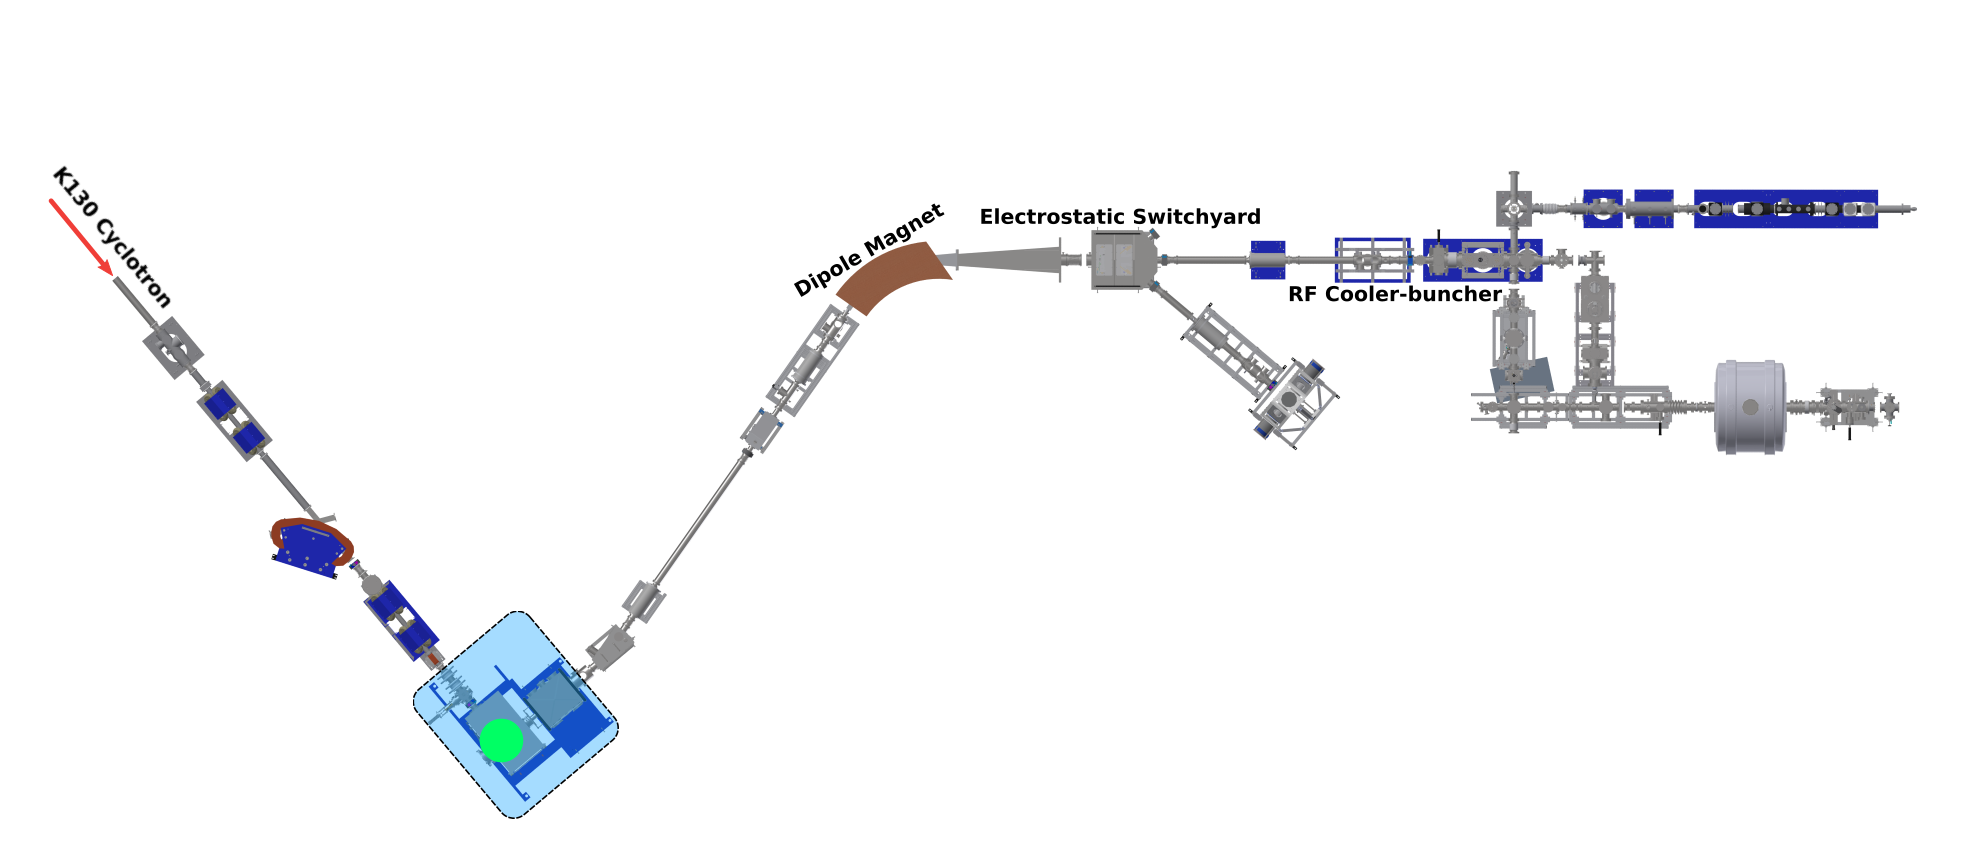
\includegraphics[width=\textwidth]{Igisol_scheme_TG.png}}%
		% \only<1->{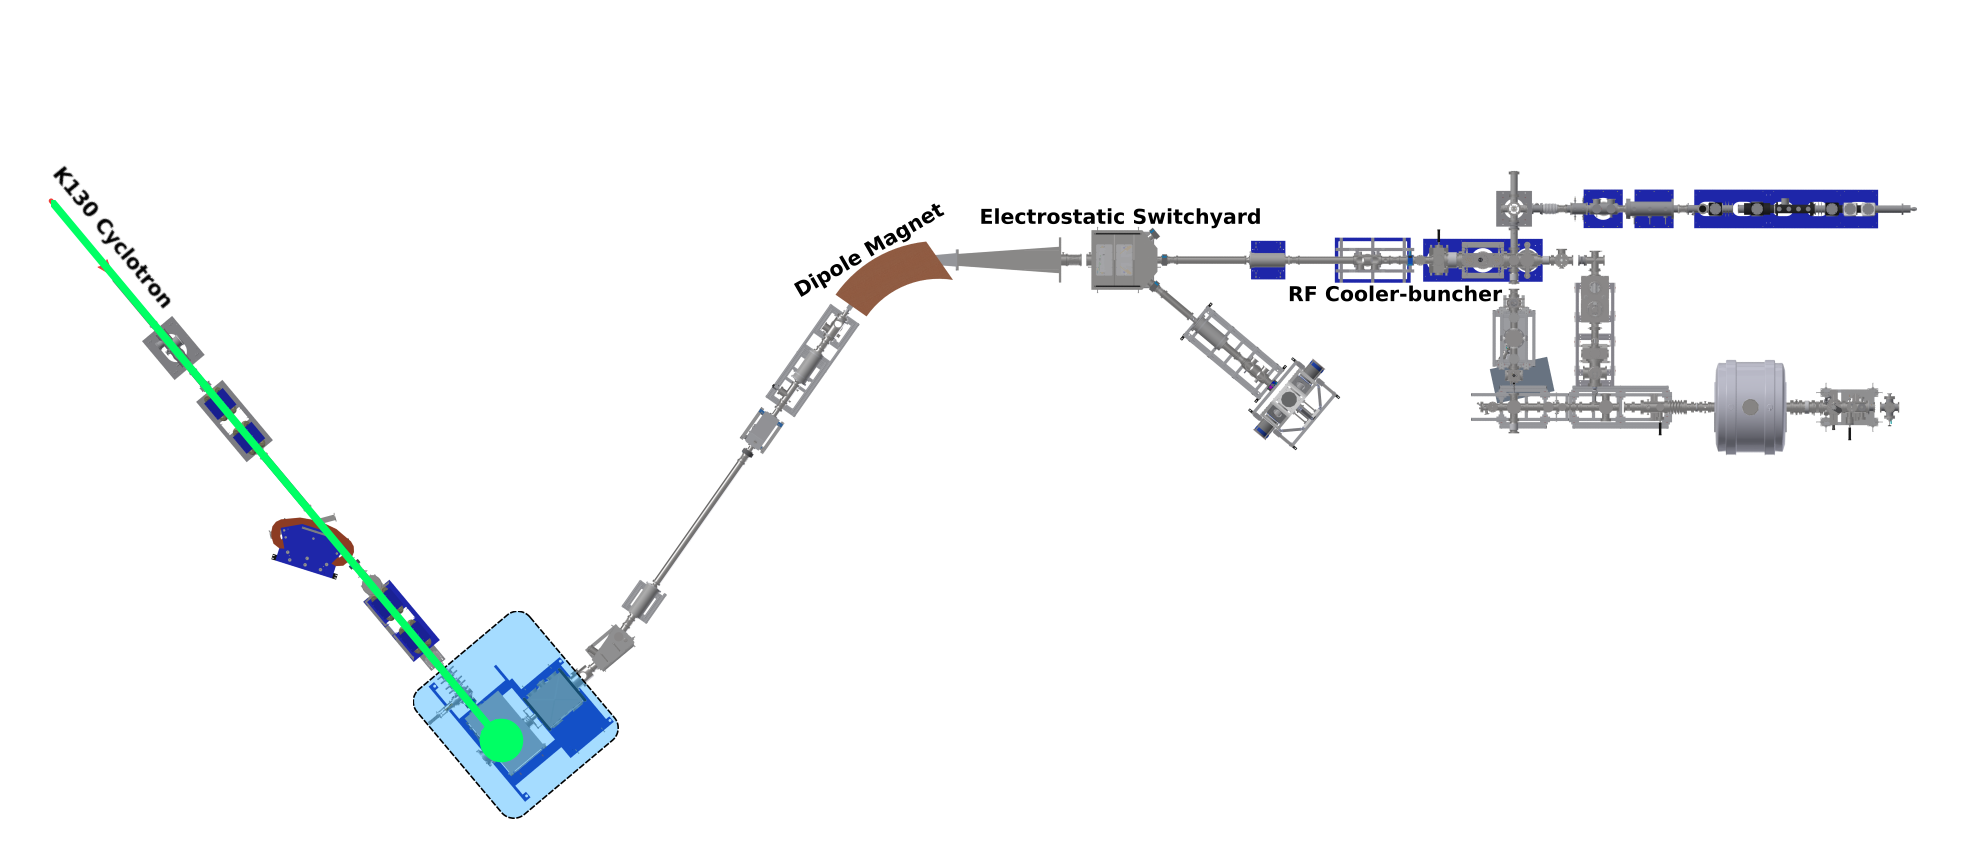
\includegraphics[width=\textwidth]{Igisol_scheme_TG_online.png}}%
		\only<1>{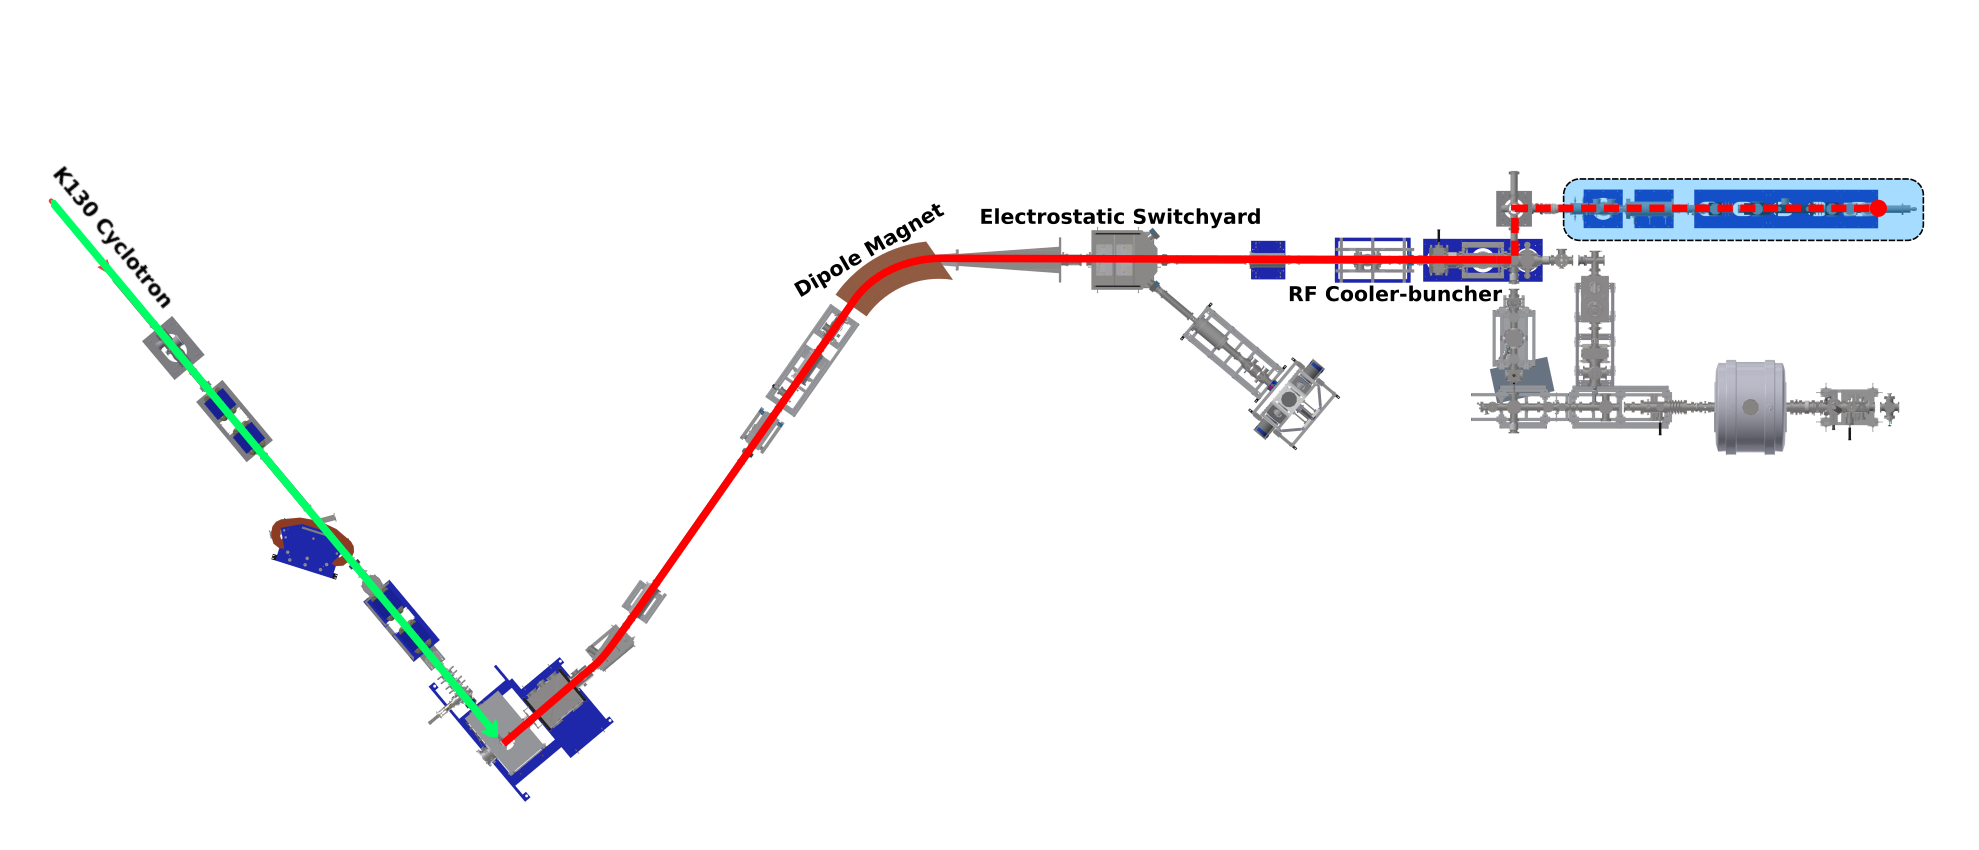
\includegraphics[width=\textwidth]{Igisol_scheme_CLS.png}}%
		% \only<5>{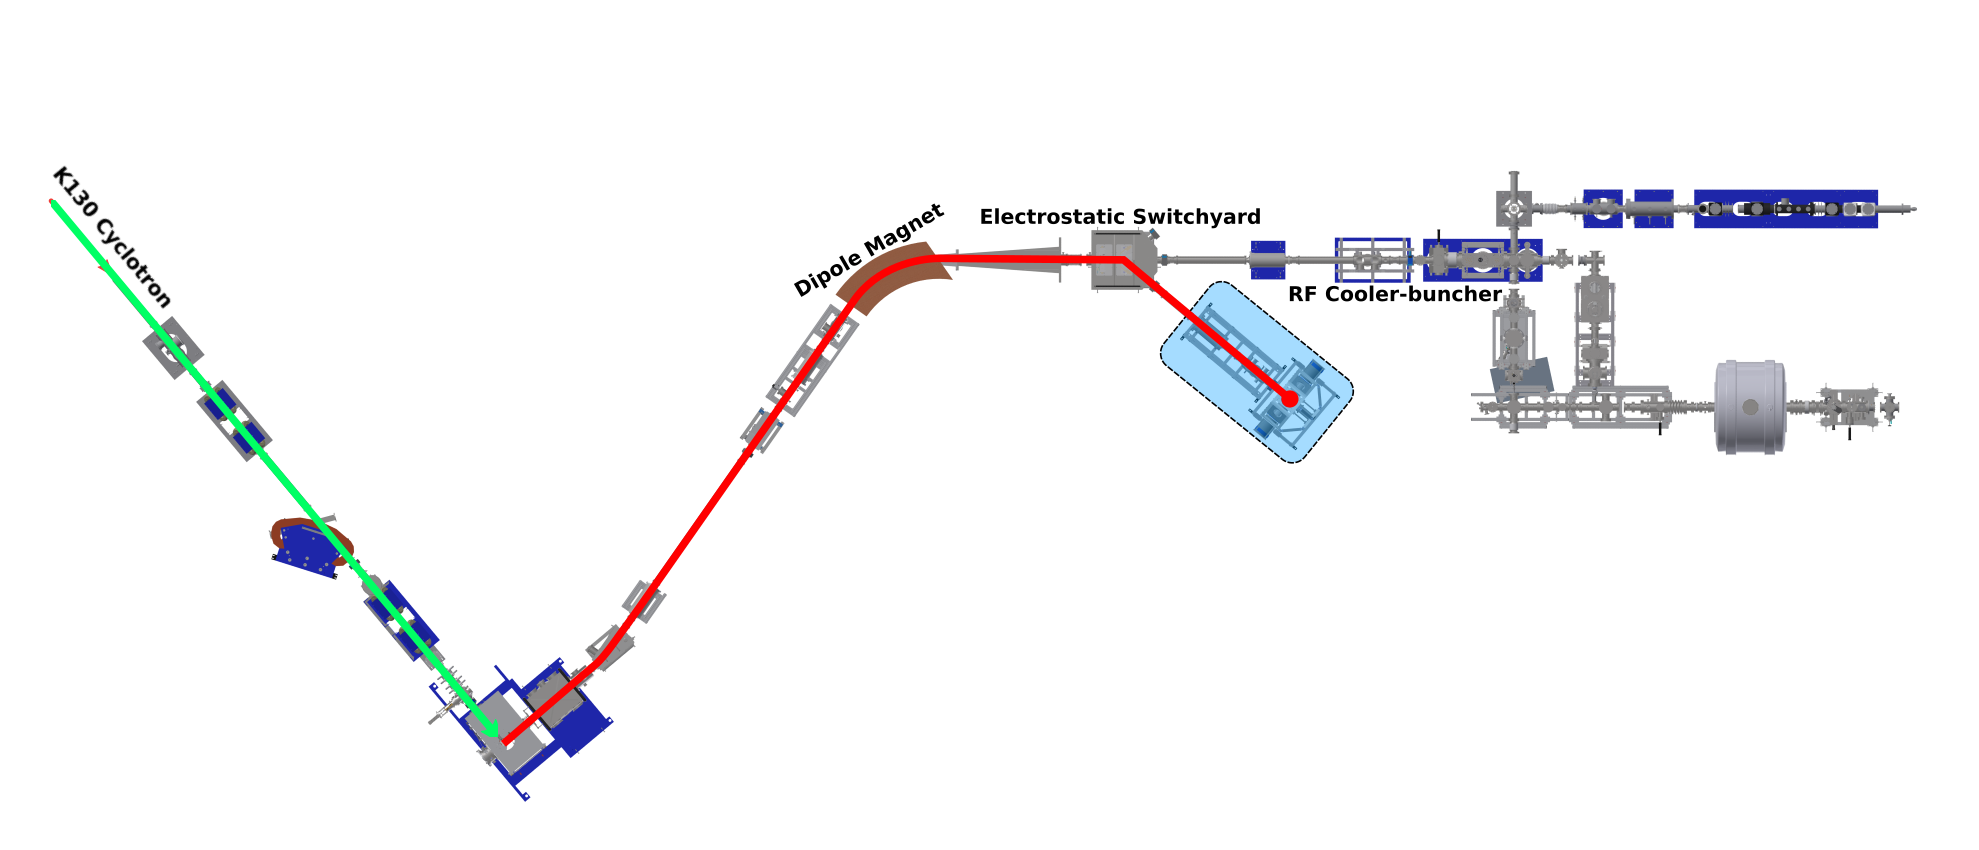
\includegraphics[width=\textwidth]{Igisol_scheme_Spec.png}}%
		% \only<6>{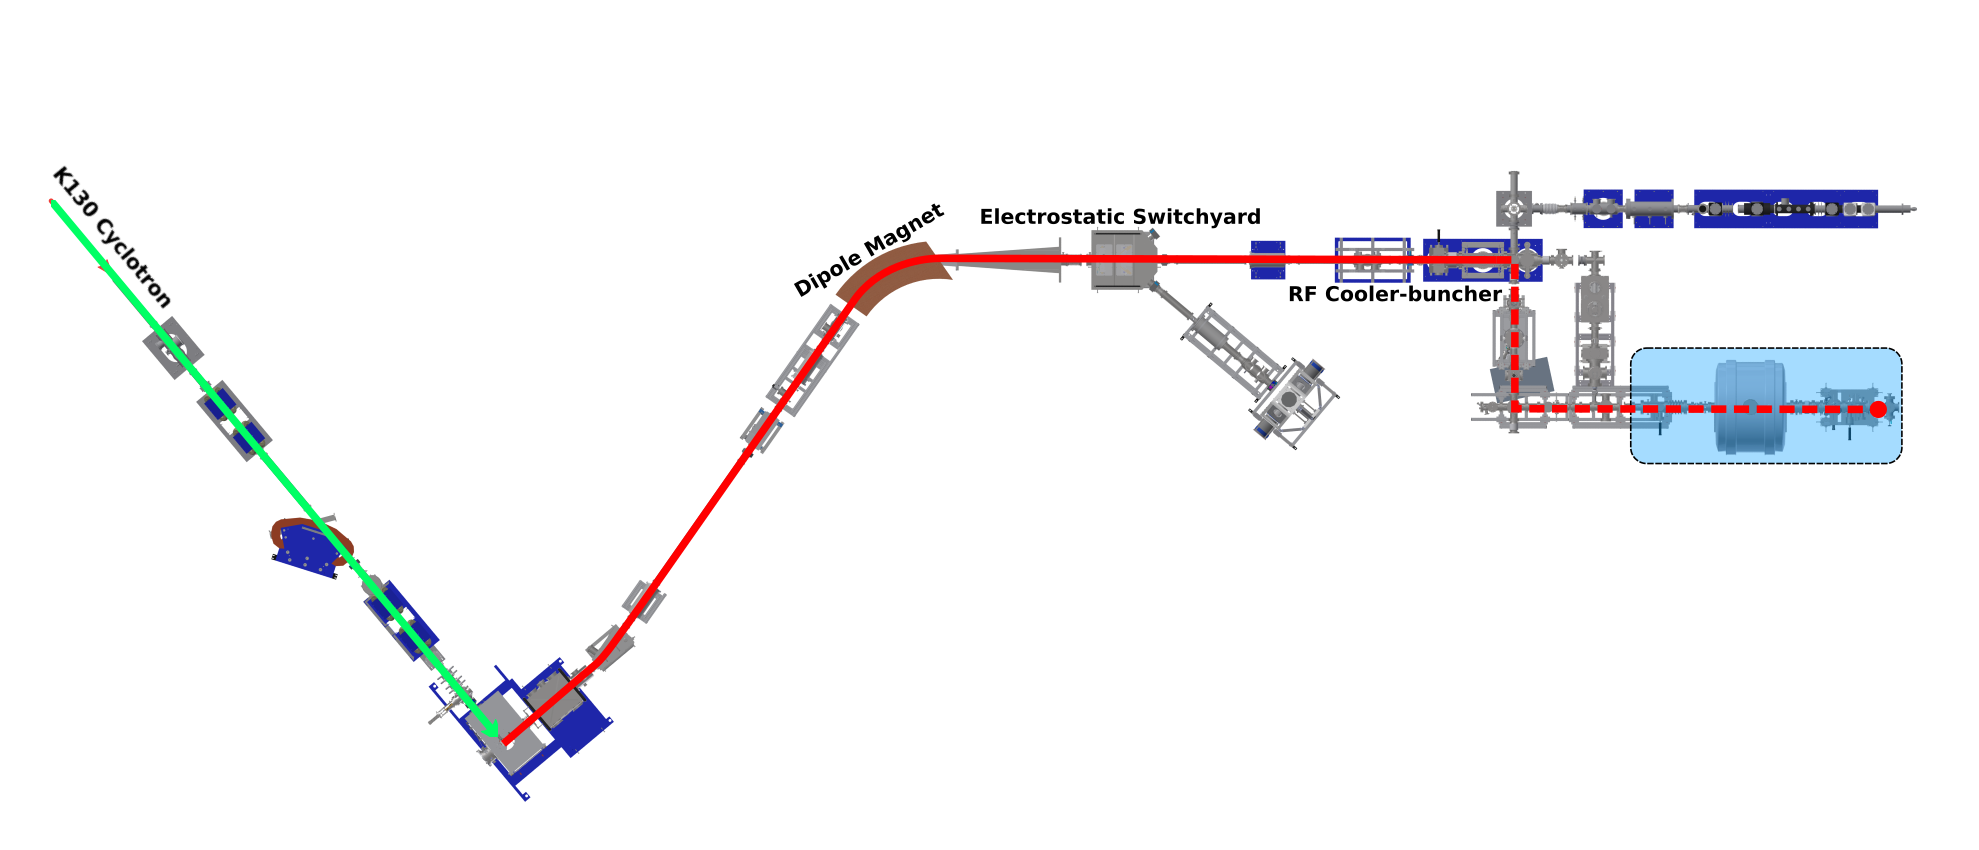
\includegraphics[width=\textwidth]{Igisol_scheme_Penn.png}}%
	\end{textblock*}
	\only<1>{


		\begin{textblock*}{0.4\paperwidth}(0.4\paperwidth,0.45\paperheight)
			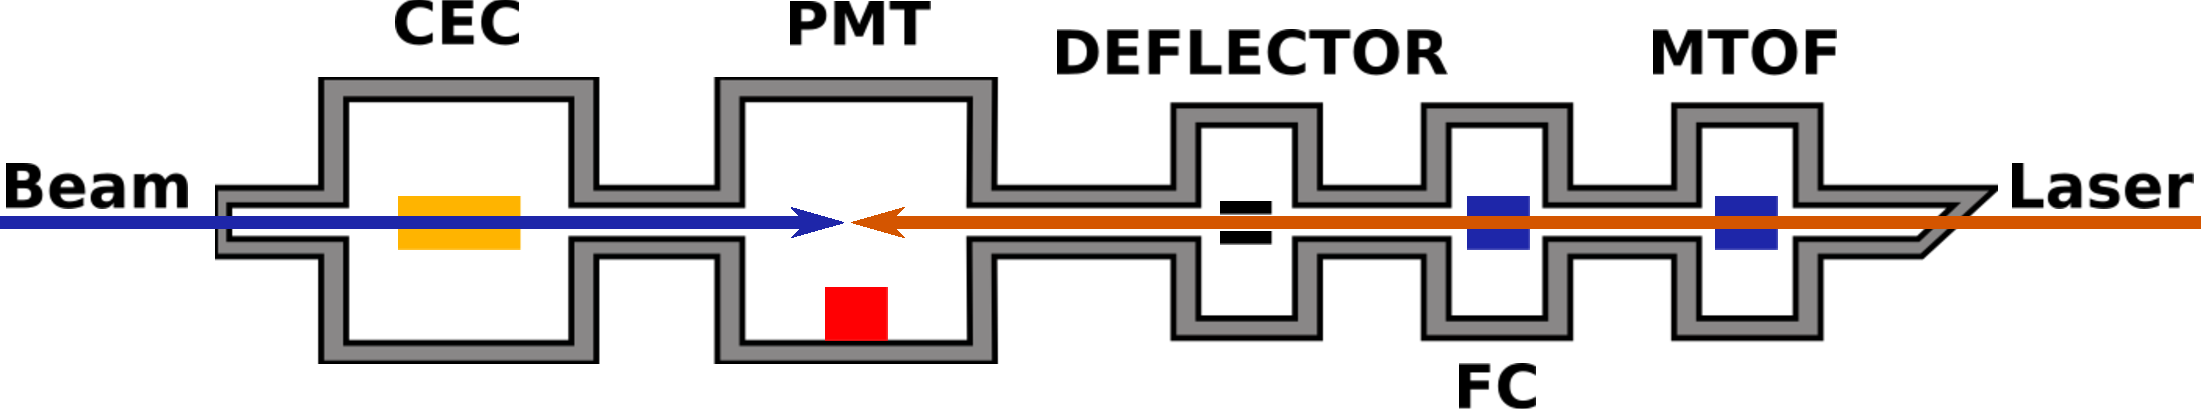
\includegraphics[width=\textwidth]{CLS.pdf}

		\end{textblock*}

		
	}
	
\end{frame}
\end{document}